
\chapter{Automatic Detection of InSAR Surface Deformation Signals In the Presence Severe Tropospheric Noise}
\label{CHAP:6-blob}
% ABSTRACT
%In this chapter, we demonstrate methods for automatically detecting surface deformation signals in InSAR maps. We present a computer vision algorithm based on Laplacian of Gaussian filters. We show how the tropospheric noise levels can be estimated from InSAR data, and we use these estimates to simulate new instances of noise. We create confidence measures based on the simulations for automatically detected signals in real InSAR maps.

Automatic detection of surface deformation features from a large volume of Interferometric Synthetic Aperture Radar (InSAR) data is challenging, because the magnitude of InSAR measurement noise varies substantially in both space and time. In this chapter, we present a computer vision algorithm based on Laplacian of Gaussian (LoG) filtering for detecting the size and location of unknown surface deformation features. Because our algorithm detects spatially coherent ``blob-like'' features, tropospheric noise artifacts that share similar spatial characteristics may also be detected. We estimate the tropospheric noise spectrum directly from data, which allows us to simulate new instances of noise that resemble the actual InSAR observations. Based on these simulations, we quantify the likelihood that a detected feature is a real deformation signal. We demonstrate the performance of our algorithm using 
ascending and descending Sentinel-1 data from Chapter \ref{CHAP:4-GRL} acquired between 2014 and 2019
%ascending and descending Sentinel-1 data acquired between 2014 and 2019 over the $\sim$ 80,000 km$^2$ oil-producing Permian Basin in West Texas, one of the most productive oil fields in the world. 
We detect clusters of deformation features associated with oil production, wastewater injection, and fault activities. The number of detected deformation features increases substantially over the study period, which is consistent with the overall rise in oil production within the Permian Basin since 2014. 
%Our algorithm is robust and flexible, which can be readily integrated to various multi-temporal InSAR time series methods for detecting a broad range of deformation features.


%\section{Introduction}
%\label{sec:ch6-intro}


% FINAL INTRO
%Interferometric Synthetic Aperture Radar (InSAR) has made it possible to monitor surface deformation with 10s–100s meter spatial resolution and millimeter-to-centimeter accuracy (e.g. \citep{Pritchard2004InSARbasedsurvey,  Chaussard2014PredictabilityHydraulicHead,  Chen20142010SlowSlip, Biggs2017GlobalVolcanoMonitoring, Chen2016ConfinedAquiferHead, Fielding2017SurfaceDeformationNorth, Chen2019TriggeringMw7.2}). Since the launch of the Sentinel-1 mission in 2014, the quantity and quality of open-access InSAR data has grown exponentially. 
%Processing and interpreting such data often requires artificial intelligence and computer vision algorithms without extensive manual inspection. However, designing robust and scalable computer vision algorithms for automatic detection of InSAR surface deformation features is challenging. This is because InSAR measurement noise varies substantially in both space and time, and its magnitude is often comparable or larger than subtle deformation signals of interest. In particular, residual troposphere noise in InSAR surface deformation maps are spatially coherent, and it can often be visually mistaken as real surface deformation.


%To address these challenges, previous studies developed algorithms for detecting deformation signals in pixel-wise InSAR deformation time series based on certain magnitude thresholds. The thresholds can be set manually \citep{Raspini2018ContinuousSemiAutomatic}, set using pixel-wise standard deviations \citep{Bekaert2020InsarBasedDetection}, derived from auxiliary data sources (e.g. global atmospheric weather models \citep{Parker2015SystematicAssessmentAtmospheric}, MODIS water vapor measurements \citep{Barnhart2013CharacterizingEstimatingNoise}), or derived from simulated noise parameters \citep{Havazli2021DetectionThresholdEstimates}. Principal component analysis (PCA) and independent component analysis (ICA) have also been used to explore decompositions of noisy time series data \citep{Chaussard2014PredictabilityHydraulicHead, Ebmeier2016ApplicationIndependentComponent, Gaddes2018BlindSignalSeparation}. Moreover, deep learning methods using convolutional neural networks (CNNs) have been applied to detect deformation features in individual interferograms \citep{Anantrasirichai2018ApplicationMachineLearning, Anantrasirichai2019ApplicationConvolutionalNeural} or InSAR time series \citep{RouetLeduc2021AutonomousExtractionMillimeter}. Because the detection problems are posed as a supervised learning task, they require either labeled training data \citep{Anantrasirichai2018ApplicationMachineLearning} or ground truth examples from simulated noise and deformation models \citep{Anantrasirichai2019DeepLearningApproach, RouetLeduc2021AutonomousExtractionMillimeter}. These supervised learning approaches work well when deformation signals of interest show spatial signatures that are distinct from InSAR measurement noise. In many applications, both deformation signals and tropospheric turbulence noise are spatially coherent ``blob-like'' features that look similar to human eyes.



%Automatic detection algorithms need to quantify the detection uncertainty based on the noise magnitude of a particular radar dataset. Auxiliary tropospheric data sources such as MODIS or weather models typically do not have sufficient spatial resolution to capture localized tropospheric turbulence noise at sub-kilometer scale. Here we present a new computer vision algorithm for detecting the size and location of unknown deformation features from a large volume of InSAR data. This algorithm is based on Laplacian of Gaussian (LoG) filters, which have been employed in the computer vision literature to detect repeatable image feature points at many scales (e.g. the Scale Invariant Feature Transform (SIFT) algorithm) \citep{Witkin1987ScaleSpaceFiltering, Lindeberg1998FeatureDetectionAutomatic, Lowe2004DistinctiveImageFeatures}. To determine whether a detected feature is associated with tropospheric artifacts, we estimate the tropospheric turbulence noise directly from InSAR data \citep{Tymofyeyeva2015MitigationAtmosphericPhase}. We analyze the tropospheric noise spectrum, and quantify the detection uncertainty based on tropospheric noise simulations that resemble the actual InSAR observations over the study area \citep{Hanssen2001RadarInterferometryData}. Our algorithm is flexible, and it can be integrated with different time series techniques to detect a broad range of deformation features.






\section{Algorithm}
\label{sec:methods}

\subsection{Automatic Feature Detection}
\label{subsec:methods-1-log}

Given a surface deformation map $M$ derived from InSAR data, the value $ M_{ij} $ at the $i^{th}$ row and $j^{th}$ column represents the magnitude of a cumulative, seasonal, or transient deformation signal at this pixel. Because the earth can be considered as a stratified elastic-viscoelastic medium, surface deformation features are often spatially coherent \citep{Segall2010EarthquakeVolcanoDeformation}. In this study, our goal is to automatically detect these features in an InSAR deformation map $M$ that covers a very large region (Algorithm 1).

There have been many computer vision algorithms that were designed to automatically detect spatially coherent ``blob-like'' features in 2D image data \citep{Lindeberg1993DetectingSalientBlob, Lindeberg1998FeatureDetectionAutomatic, Lowe2004DistinctiveImageFeatures}. In this study, we employ the Laplacian of Gaussian (LoG) filters as a blob detector. An LoG kernel $K^{(m)}$ with a size $\sigma_m$ is written as:
\begin{equation}
	K^{(m)}_{ij} = \left(\frac{(i - l)^2 + (j - l)^2 - 2\sigma_m^2}{2 \pi \sigma_m^4}\right) \, e^{-\frac{ (i - l)^2 + (j - l)^2}{2 \sigma_m^2}} \label{eq:log-kernel}
\end{equation}
where pixel indices $ij  \in \left\lbrace 0, 1, \ldots, 2l \right\rbrace$. The unit of $\sigma_m$ is given in pixels, which can be scaled to meters based on the pixel spacing of the InSAR deformation map $M$.



\begin{figure}
	\centering
	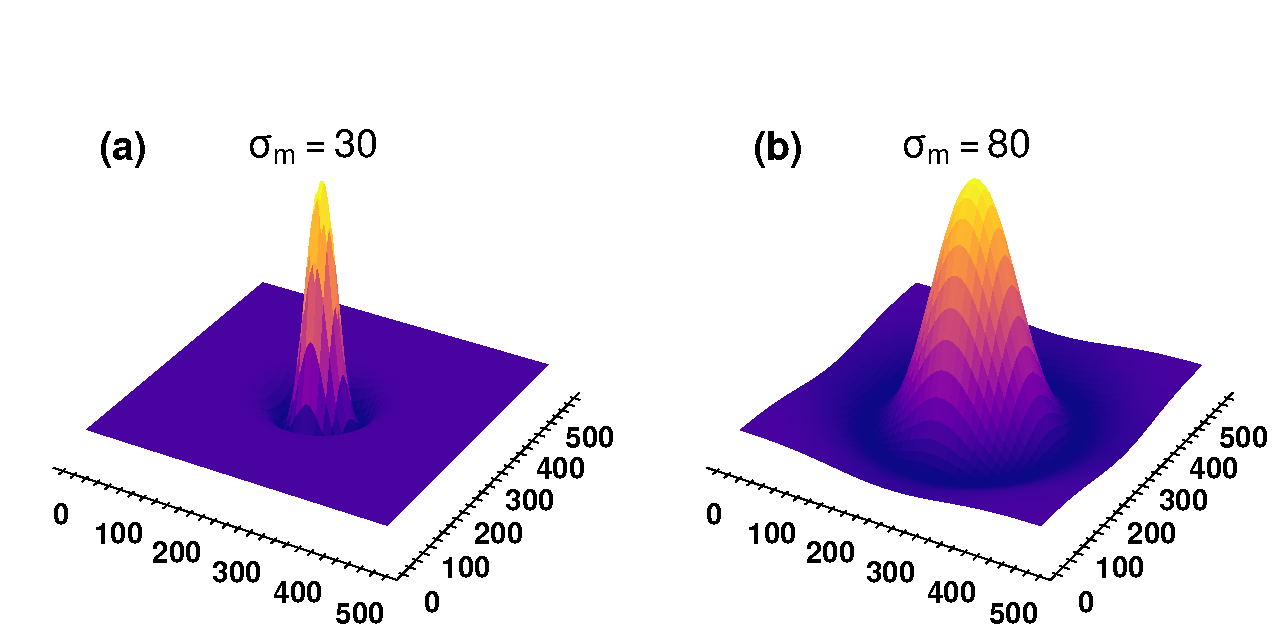
\includegraphics[width=0.95\linewidth]{figures/chapter6-blobs/figure1_log_examples.pdf}
	\caption[LoG kernel examples]{
		Laplacian of Gaussian (LoG) kernels with (a) $\sigma_m=30$ pixels and (b) $\sigma_m=80$ pixels for an image of size of 500-by-500 pixels.
	}
	\label{fig:log-kernel}
	%
\end{figure}



We generate a set of LoG kernels $K^{(1)}, K^{(2)}, \ldots$ with progressively larger $\sigma_m$ (Figure \ref{fig:log-kernel}), and calculate the $m^{th}$ filter response $ L^{(m)} $ as:
\begin{equation}
	L^{(m)} = M \ast K^{(m)}  \label{eq:log-layer-conv}
\end{equation}
%However, this operation is computationally expensive for larger kernels; thus, the filtering is carried out in the Fourier domain.
Here $*$ denotes the 2D discrete convolution, which is typically computed using the Fast Fourier Transform (FFT) algorithm because of its superior computational efficiency \citep{Szeliski2022ComputerVision}.



\begin{figure}
	\centering
	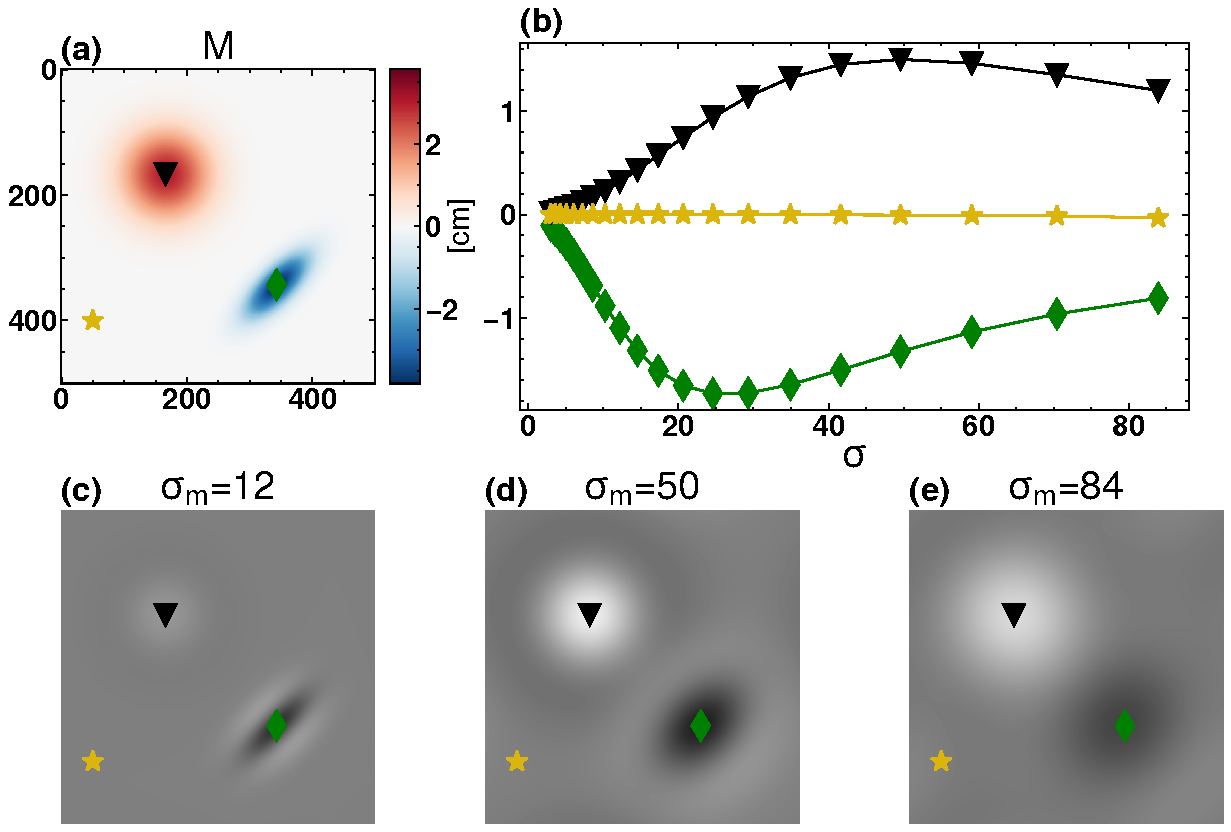
\includegraphics[width=0.98\linewidth]{figures/chapter6-blobs/figure2_log_response.pdf}
	\caption[Example LoG filter responses for synthetic deformation]{
		(a) A synthetic deformation map that contains one Gaussian-shaped uplift feature in the upper left and one elliptical Gaussian subsidence feature in the lower right. (b) LoG response amplitudes for 20 filters with various sizes ($\sigma_m$) at three marker points. The marker locations are shown in panel (a). (c)-(e) The LoG filter responses for $\sigma_m=$ 12, 50, and 84.}
	\label{fig:log-response}
	%
\end{figure}


To demonstrate how to estimate the size of an unknown deformation feature from the filter responses, Figure \ref{fig:log-response} (a) shows a $500 \times 500$ synthetic deformation map $M$ that contains one Gaussian-shaped uplift feature in the upper left and one elliptical Gaussian subsidence feature in the lower right. We filtered this deformation map using 20 LoG kernels of sizes ranging from $\sigma_1 = 3$ pixels to $\sigma_{20} = 100$ pixels with a base-2 logarithmic spacing, and the filter responses are shown in Figure \ref{fig:log-response} (b)-(e). For the round uplift case, the filter response $L^{(m)}$ (the black curve in Figure \ref{fig:log-response} (b)) is strongest when the kernel size $\sigma_m$ matches the deformation feature radius $r$ as $r = \sqrt{2}\sigma_m$. This is known as the extreme point, or the local maximum points of $|L^{(m)}|$ for all attempted $\sigma_m$. For the elliptical subsidence case, the extreme point is reached when the average length of the two primary axes of the deformation feature is $\sim \sqrt{2}\sigma_m$ (the green curve in Figure \ref{fig:log-response} (b)). For the case of no deformation, no substantial filter response is generated for any filter size (the gold curve in Figure \ref{fig:log-response} (b)).



In the case that two candidate blobs have more than 50\% overlapping area, the blob with a smaller size is discarded. 
Additionally, the LoG filter may falsely flag ghost blobs at the edges of real deformation features. This is because deformation features with strong curvature at the center also contain a strong opposite-signed curvature near the border \citep{Lindeberg1998FeatureDetectionAutomatic}. To remove those false positives, we use the distance from the candidate blob's center location to the nearest deformation amplitude extremum as a measure. If this distance is close to the blob radius, the detection is likely a ghost blob. In our test case, we discarded blobs with local extremum distances larger than 75$\%$ of the blob radius, which effectively removed all visible false positives near the edge of real deformation features.

For the $k^{th}$ detected deformation feature, our algorithm outputs the blob center location $(i_k, j_k)$, the blob radius $ r_k$, the filter response magnitude $|g_k|$ at the extreme point, and the deformation magnitude $|\bar{d_k}|$ defined as the weighed maximum of all pixels within the $k^{th}$ blob:
\begin{equation}
	\bar{d_k} = \max_{kk} |w_{kk} M_{kk} | 
\end{equation}
Here the weight $w_{kk}$ equals $\exp\left[-(r_{kk} / r_k)^2\right]$, where $r_{kk}$ is the distance between a pixel within the blob and the blob center. The exponential weighting prevents pixel outliers from distorting the measure of feature magnitude. 

We can exclude undesired deformation features by setting magnitude thresholds on $|g_k|$ and $|\bar{d_k}|$ based on users' interest. Furthermore, we need to determine whether a detected deformation feature has a signal magnitude above the noise level of the InSAR deformation map, which is the focus of the following method sections. 


\begin{algorithm}
	\caption{LoG Based Deformation Feature Detection}\label{algo:blobs}
	\SetAlgoLined
	\KwIn{2D InSAR deformation map $M$}
	\KwResult{For each $k \in {1, \ldots, N_d}$ detections, the algorithm outputs the blob center location $ (i_k,j_k) $, the blob radius $ r_k $, the filter response magnitude $|g_k|$ at the extreme point, the deformation magnitude $|\bar{d_k}|$ }
	
	
	// Calculate filter responses:\\
	\ForEach{$ \sigma_m \in \left\lbrace \sigma_{min} \ldots \sigma_{max}\right\rbrace $}{
		%$L^{(n)} = \mathcal{F}^{-1} \left[ \mathcal{F} M \cdot  \mathcal{F} K^{(n)} \right] $
		$ L^{(m)} = M \ast K^{(m)}  $
		%$\nabla^2_{norm} L(\cdot, \cdot, \sigma) \gets I(\cdot, \cdot) * \nabla^2_{norm} G(\cdot,\cdot, \sigma)$
	}
	
	// Find candidate blobs from local extrema:\\
	\For{$ (i, j, m) \in  L $}{
		\If{$L[i, j, m] $ is local extremum }{
			% \If{$\det \mathcal{H}_{norm} L(x,y,\sigma ) $ is local extremum }{
				Compute $ r = \sqrt{2}\sigma_m $ \\
				Add $ (i, j, r) $ to list of candidate detections
		}
	}
	// Prune blobs with overlap:\\
	\ForEach{$ b_1 := (i_1, j_1, r_1), b2 := (i_2, j_2, r_2) \in $ candidates}{
		%	Form circle of radius $ r_i $ around $ (i_1, j_1) $\\
		\If{ Overlap$( b_1, b_2 ) > 0.5 $  }{
			Remove smaller of $ b_1, b_2 $
		}
	}
	
	// Prune edge blob false positives:\\
	\ForEach{$ b_k := (i_k, j_k, \sigma_k) \in $ candidates}{
		Find coordinates $(u, v)$ of local max of $M$ within
		radius $r_k$ around $ (i_k, j_k) $
		\\
		\If{ $\sqrt{(x - u)^2 + (y - v)^2} > 0.75 $  }{
			Discard $ b_k $
		}
	}
	// Prune with thresholds $ \gamma_g, \gamma_d $:\\
	\ForEach{$ b_k := (i_k, j_k, r_k,|g_k|, |\bar{d_k}|) \in $ candidates}{
		\If{ $ |g_k| <  \gamma_g $ \text{or} $ |\bar{d_k}| <  \gamma_d $  }{
			Discard $ b_k $
		}
	}
\end{algorithm}



\subsection{Tropospheric Noise Spectrum}
\label{sec:ch6-methods-2-tropo-spectrum}
InSAR measurement noise can also produce spatially coherent "blob-like" features that are detectable by our algorithm.  Here we focus on characterizing the tropospheric turbulence noise in each SAR scene. This is because tropospheric turbulent noise (1) is correlated in space \citep{Emardson2003NeutralAtmosphericDelay, Lohman2005SomeThoughtsUse}; (2) is present in all InSAR data sets with greatly varying magnitudes \citep{Barnhart2013CharacterizingEstimatingNoise, Hooper2012RecentAdvancesSar}; and (3) is often the primary noise source that limits InSAR measurement accuracy \citep{Jolivet2014ImprovingInsarGeodesy, Bekaert2015StatisticalComparisonInsar, Parker2015SystematicAssessmentAtmospheric}.

Consider an interferogram formed using two SAR scenes acquired at times $t_1$ and $t_2$. In the case that tropospheric turbulence noise is the dominant noise term, the measured interferometric phase $\phi_{1,2}$ (in radians) at a pixel of interest can be written as \citep{Zebker1997AtmosphericEffectsInterferometric}:
\begin{equation}
	\phi_{1,2} \approx \frac{4 \pi}{\lambda} \left(\alpha_2 - \alpha_1 + \Delta d_{1,2} \right)
\end{equation}
where $ \lambda $ is the radar wavelength, $\alpha_1$ and $\alpha_2$ represent the tropospheric delay at the two SAR acquisition times $t_1$ and $t_2$, and $\Delta d_{1,2} $ is the Line-Of-Sight (LOS) deformation ($d_2-d_1$) between $t_1$ and $t_2$. The unit of $\lambda$, $\alpha_1$, $\alpha_2$, and $\Delta d_{1,2} $ is in centimeters. 

Given $N$ SAR acquisitions, we can estimate the tropospheric noise on the $n^{th}$ SAR acquisition date by averaging $N-1$ interferograms that share the common reference SAR scene $n$ \citep{Tymofyeyeva2015MitigationAtmosphericPhase}:
%multline not needed for single column
%\begin{multline}
%\bar{\alpha}_n = \frac{\lambda}{4 \pi} \frac{1}{N-1} \left(\sum_{k=1, k \neq n}^{N} \phi_{k,n}\right)  \\
%=  \alpha_n  + \frac{1}{N-1} \left( \sum_{k=1, k \neq n}^{N}  \Delta d_{k,n} - \sum_{k=1, k \neq n}^{N}  \alpha_k  \right)  \label{eq:avg-ifg} 
%\end{multline}
\begin{equation}
	\bar{\alpha}_n = \frac{\lambda}{4 \pi} \frac{1}{N-1} \left(\sum_{k=1, k \neq n}^{N} \phi_{k,n}\right)  
	=  \alpha_n  + \frac{1}{N-1} \left( \sum_{k=1, k \neq n}^{N}  \Delta d_{k,n} - \sum_{k=1, k \neq n}^{N}  \alpha_k  \right)  \label{eq:avg-ifg} 
\end{equation}
Because tropospheric turbulence noise is uncorrelated in time for scales longer than one day \citep{Emardson2003NeutralAtmosphericDelay, Onn2006ModelingWaterVapor}, the term $ \frac{1}{N-1} \sum \alpha_k \rightarrow 0$ when $N$ is sufficiently large. 
Under the assumption that $ \frac{1}{N-1} \sum \Delta d_{k,n} $ is relatively small comparing to $\alpha_n$, we compute $ \bar{\alpha}_n $ at each pixel to obtain a tropospheric turbulence noise map $A^{(n)}$ for the $n^{th}$ SAR acquisition date over the entire study area. In Section \ref{sec:results:path78}, we further discuss the impact of the deformation signals on our tropospheric noise analysis.


We next compute the 2D Power Spectral Density (PSD) of the $n^{th}$ tropospheric noise estimates at  wavenumber $ k_x, k_y $ (with units $1/m$) as \citep{Jacobs2017QuantitativeCharacterizationSurface}:
\begin{equation}
	\text{PSD}_n(k_x, k_y) = \frac{| \widehat{A^{(n)}} |^2 }{N_x N_y (\frac{1}{\Delta x \Delta y}) } \label{eq:pow-spec}
\end{equation}
where  $\widehat{A^{(n)}}$ is the Discrete Fourier transform (DFT) of  the $n^{th}$ tropospheric noise map $A^{(n)}$, $\Delta x$ and $\Delta y$ are the interferogram pixel spacings (in meters) in the $x$ and $y$ directions, $N_x$ and $N_y$ are the total number of pixels in the $x$ and $y$ directions, and the squared absolute value and division are pixel-wise operations. 


As an example, Figure \ref{fig:psd-example} (a) shows a synthetic 2D tropospheric turbulence noise map. We calculate the 2D PSD of the noise map following Equation \eqref{eq:pow-spec} (Figure \ref{fig:psd-example} (b)). Under the assumption that tropospheric noise is isotropic, we average all pixels with a distance  $k= \sqrt{k_x^2 + k_y^2}$ from the origin to generate a 1D PSD as a function of $k$ \citep{Hanssen2001RadarInterferometryData}.
We plot the 1D PSD on a log-log scale, which rolls off following a power law at higher frequencies (Figure \ref{fig:psd-example} (c)). By contrast, the power spectrum of spatially uncorrelated while noise is relatively flat across all frequencies $k$ (Figure \ref{fig:psd-example} (d)-(f)).


\begin{figure}
	\centering 
	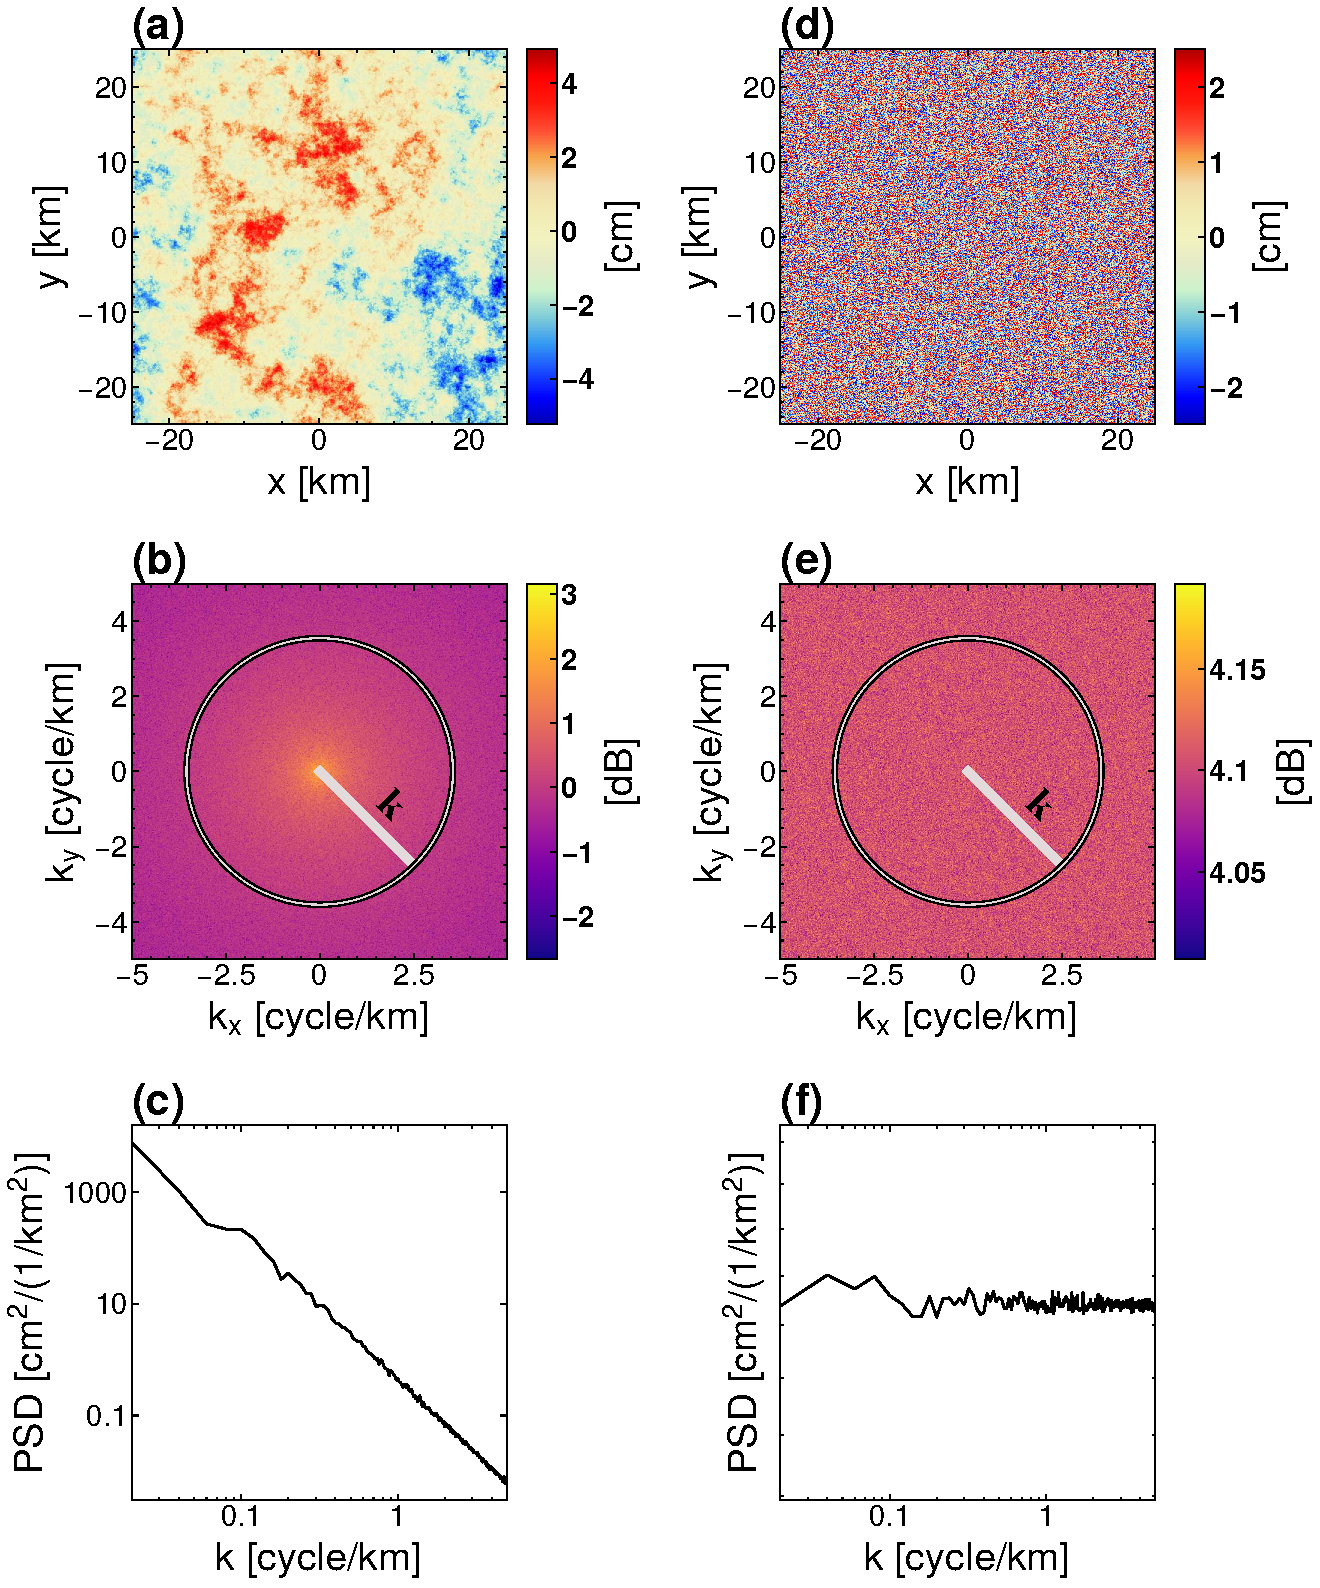
\includegraphics[width=0.90\linewidth]{figures/chapter6-blobs/figure3_psd_radial.pdf}
	%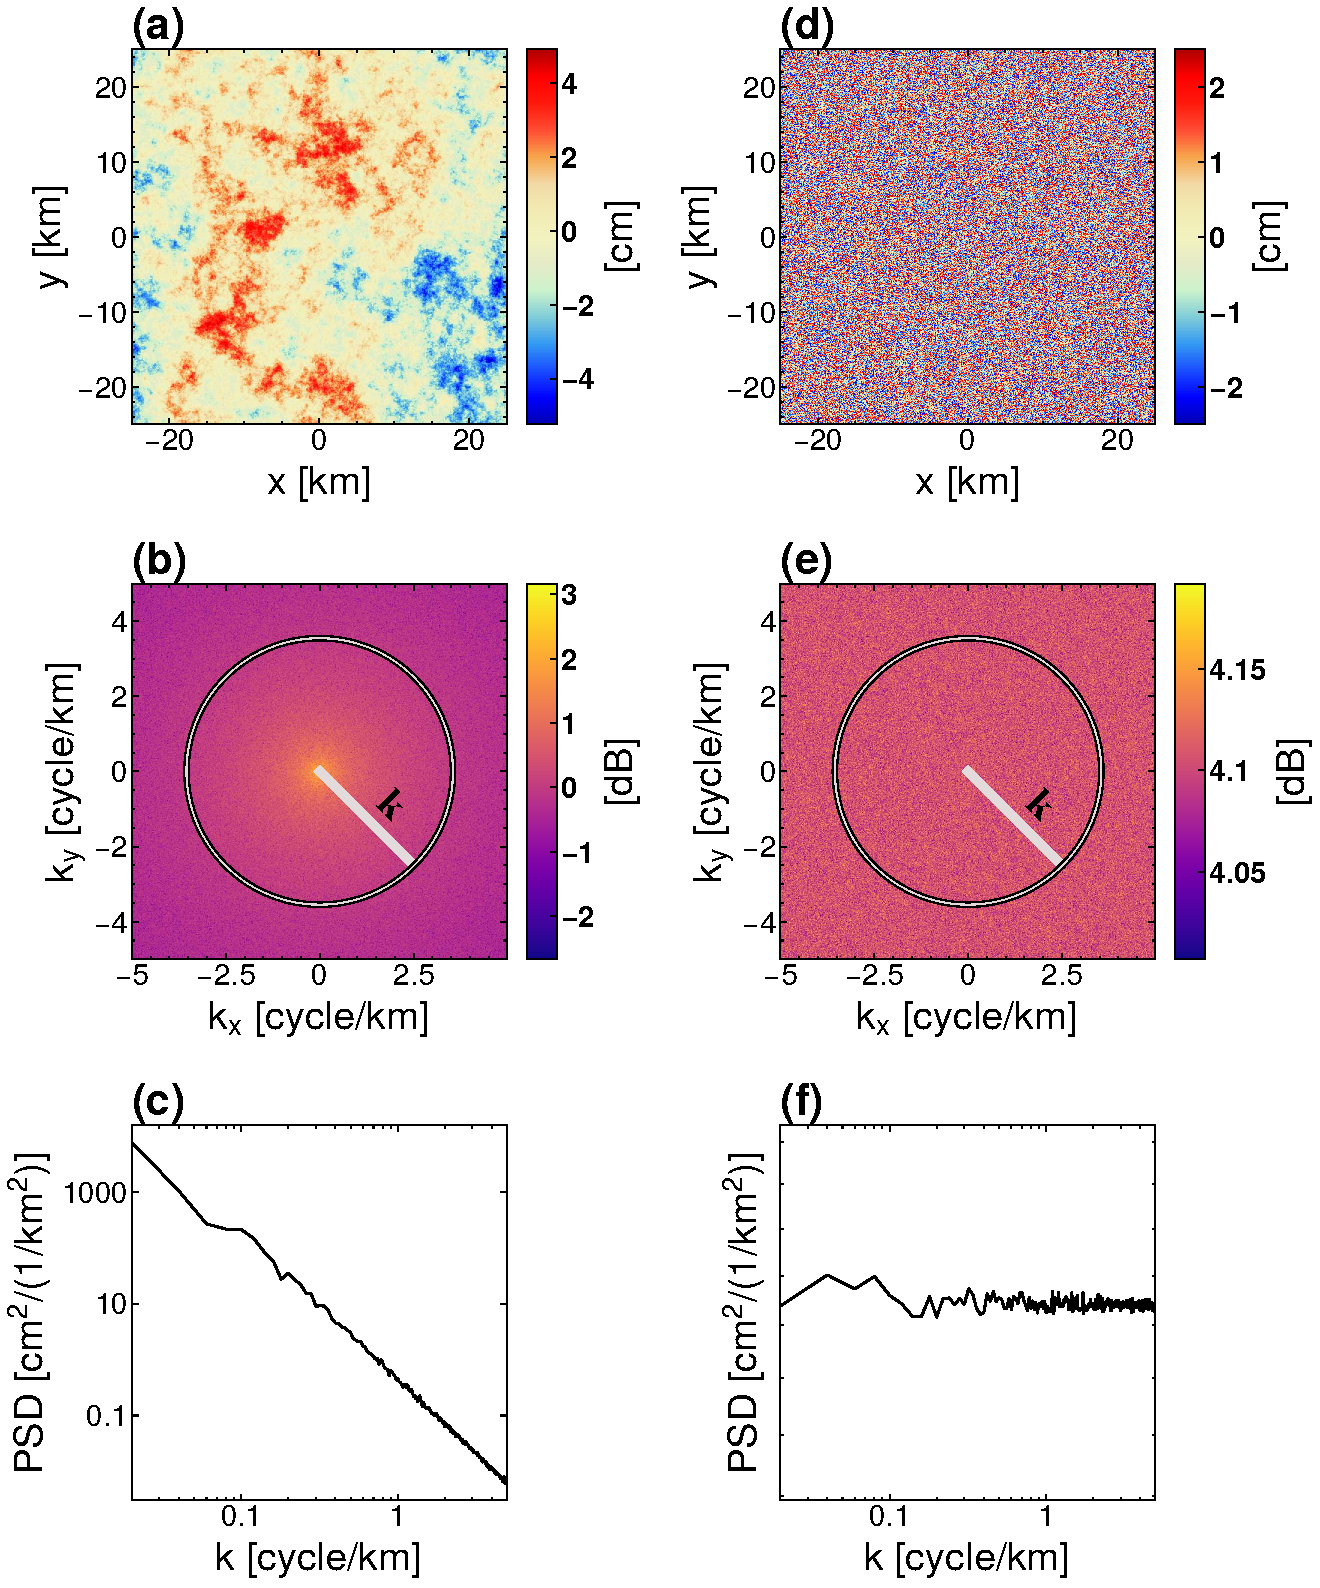
\includegraphics[width=0.98\linewidth]{figures/chapter6-blobs/figure3_psd_radial.png}
	\caption[Calculation of 1D PSDs for tropospheric noise]{
		(a) A simulated 2D turbulent atmospheric noise map with $ 500 \times 500 $ pixels at $100$ meter pixel spacing.
		(b) 2D Power Spectral Density (PSD) of the tropospheric noise map in panel (a).
		(c) 1D PSD as a function of wavenumber $k = \sqrt{k_x^2 + k_y^2}$, under the assumption that tropospheric noise is isotropic.
		(d) A simulated 2D white noise map (spatially uncorrelated) with the same dimension and pixel spacing as panel (a)
		(e) 2D PSD of the white noise map in panel (d).
		(f) 1D PSD as as a function of wavenumber $k = \sqrt{k_x^2 + k_y^2}$. Here we averaged the 1D PSD of 50 2D white noise instances to improve the statistical stability of the spectral estimates.
	}
	\label{fig:psd-example}
\end{figure}

\FloatBarrier


\subsection{Uncertainty Quantification}
\label{subsec:methods-3-noise-sim}

Using the average 1D PSD of all $N$ InSAR-observed tropospheric turbulence noise maps, we can simulate $N$ 2D noise incidences  $S^{(1)},\dots, S^{(N)} $ that closely resemble the real tropospheric noise over the study area \citep{Hanssen2001RadarInterferometryData}. Using these simulated noise maps, we form up to $N(N-1)/2$ noise-only interferograms, and derive a time series solution following the same method for generating the real InSAR deformation map $M$ (e.g. \citep{Sandwell1998PhaseGradientApproach, Berardino2002NewAlgorithmSurface}). Because these synthetic interferograms contain no deformation, any "blob-like" features in the simulated time series solution are associated with tropospheric noise. We record the radius $r_k$,  the filter response magnitude $|g_k|$ and the magnitude $|\bar{d_k}|$ of each noise feature using our automatic blob detection algorithm.

Similarly, we generate many synthetic InSAR data sets that share the same noise spectrum derived from data, and record all detected noise blobs. We create 2D histograms of the noise attributes (filter response magnitude vs. radius and deformation magnitude vs. radius), which allows us to remove candidate blob features in the real deformation map $M$ that are likely due to tropospheric noise artifacts.


\section{Test Site}
\label{sec:site}


% on over an 80,000 km$^2$ oil-producing region in the Permian Basin, West Texas.  As described in \citep{Staniewicz2020InsarRevealsComplex}, we processed 84 ascending Sentinel-1 scenes (Path 78, Frames 94–104) acquired between November 2014 and January 2019 (Figure \ref{fig:study-area}). We imposed no maximum spatial baseline and a maximum temporal baseline of 800 days for interferogram selection, resulting in 2550 multi-looked interferograms with 120 m pixel spacing.  We used the GPS station TXKM as the reference location, where little surface deformation was observed over the study period (Figure \ref{fig:study-area}, yellow dot).


%\begin{figure}[hbt!]
%	\centering
%	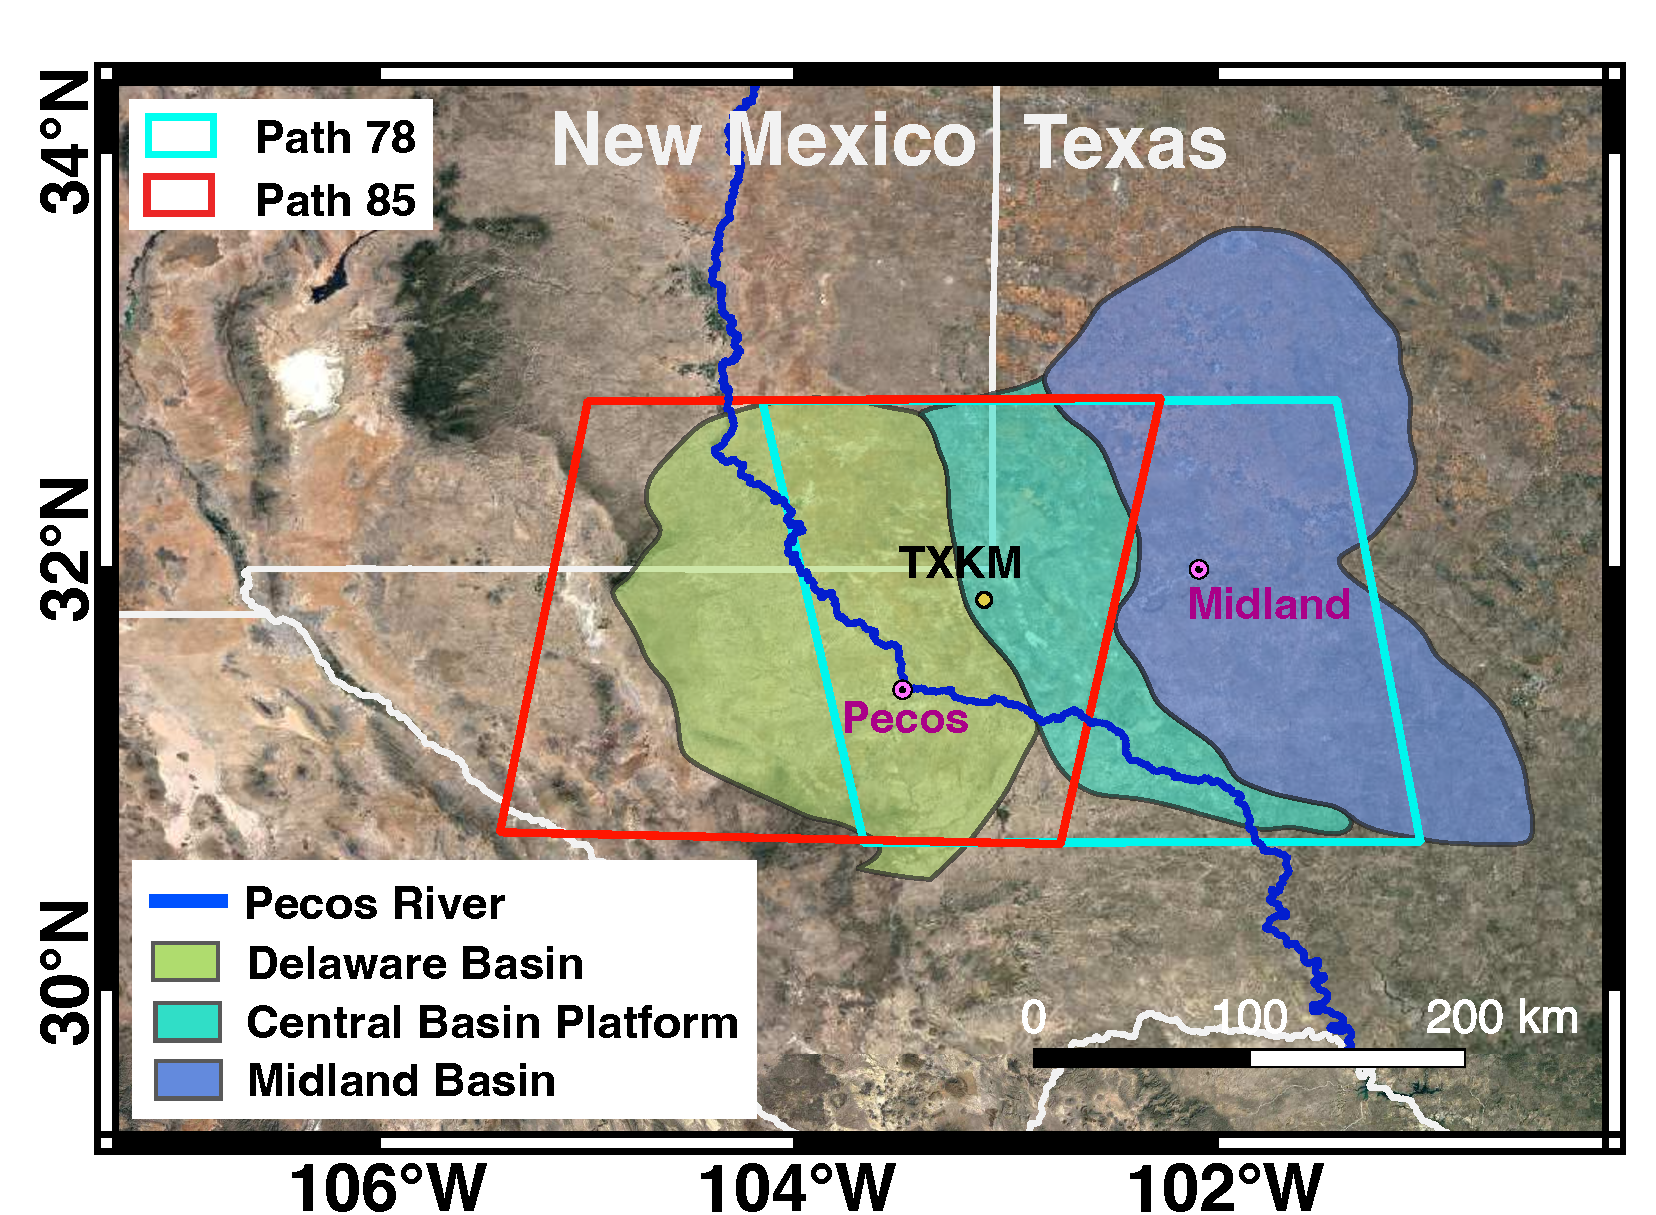
\includegraphics[width=0.59\linewidth]{figures/chapter6-blobs/figure4-study-area.pdf}
%	%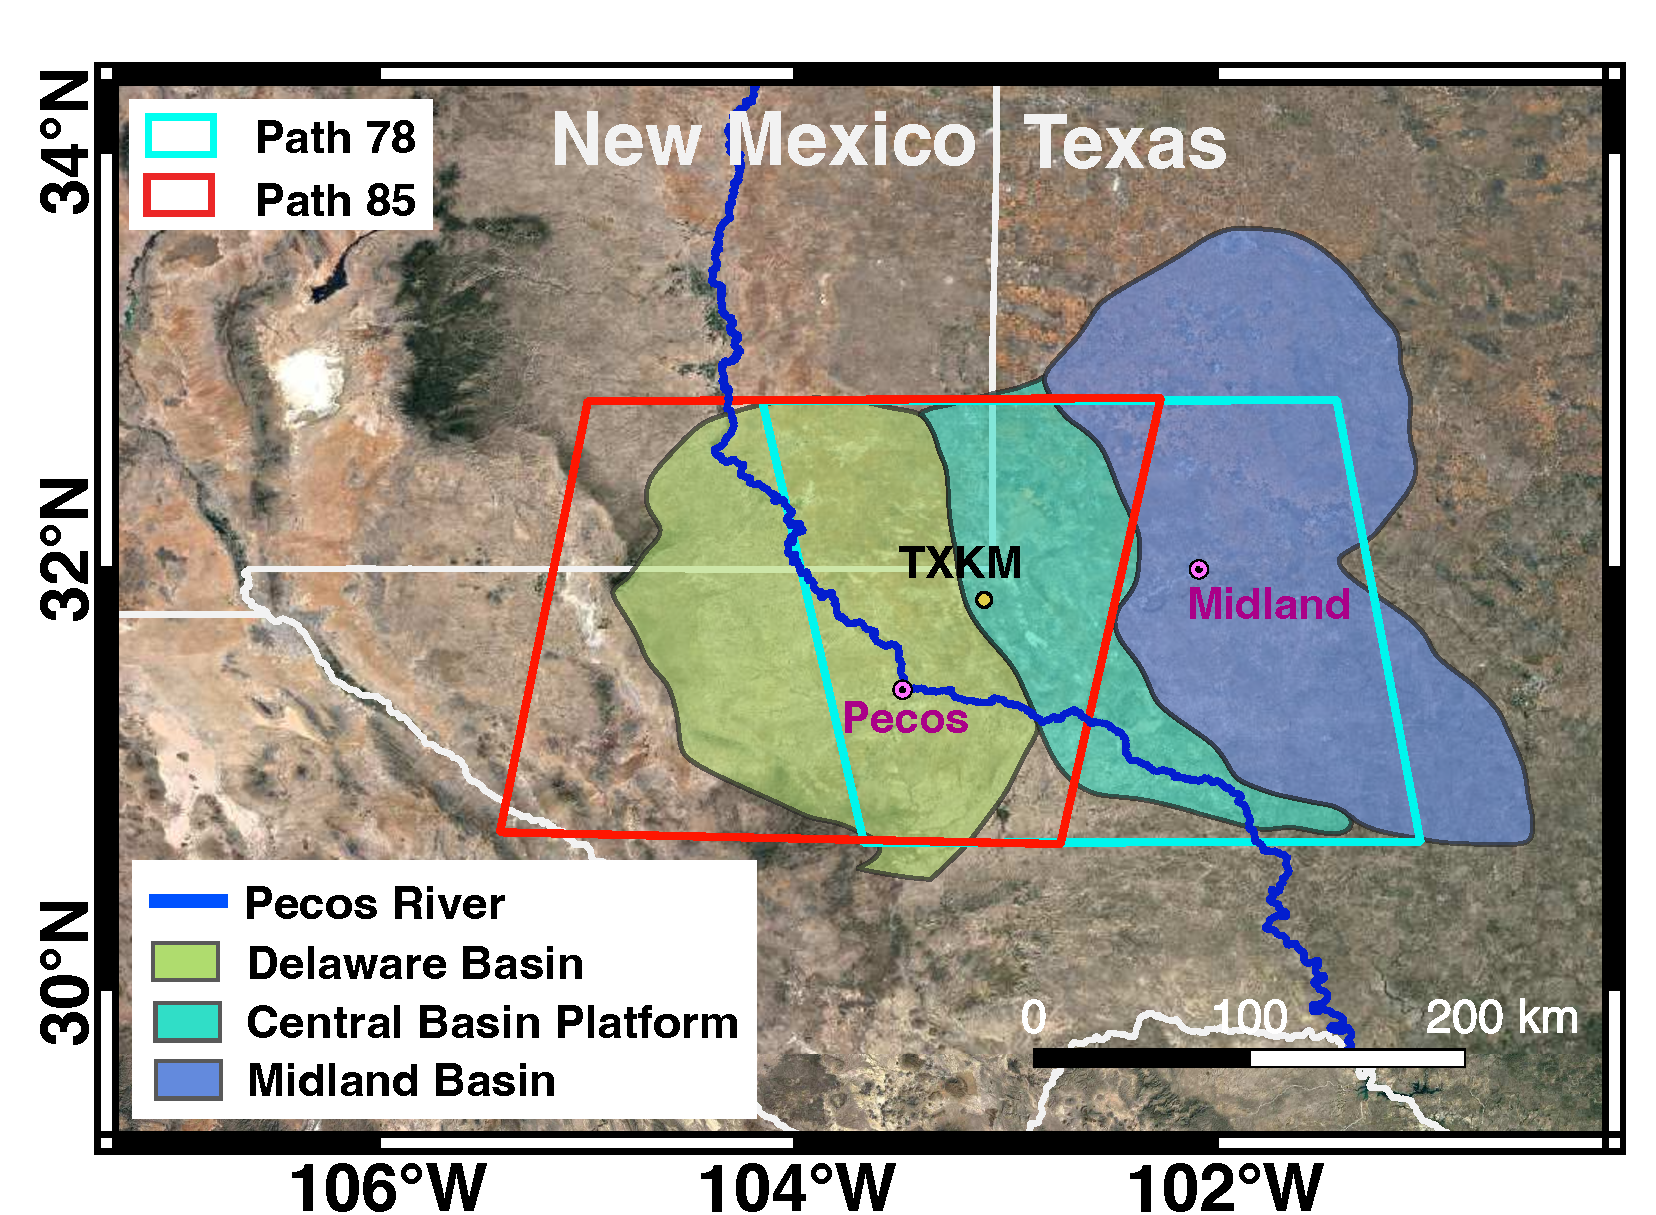
\includegraphics[width=0.96\linewidth]{figures/chapter6-blobs/figure4-study-area.png}
%	\caption{GPS and InSAR data coverage over the Permian Basin. Teal and red boxes indicate Sentinel-1 InSAR coverage for ascending Path 78 and descending Path 85. GPS station TXKM (yellow dot) was used as the reference point for both paths.
%		%Each path contains over 80 SAR acquisitions, leading to over 3500 interferograms per path at 180 m pixel spacing.
%	}
%	\label{fig:study-area}
%\end{figure}


%We employed a stacking approach \citep{Sandwell1998PhaseGradientApproach, Staniewicz2020InsarRevealsComplex} to calculate the average LOS velocity $v_{avg}$ at each ground pixel over a time period of interest $ T $ as
%\begin{equation}
%	v_{avg} = \frac{\sum_{i \in G} \Delta d_i}{\sum_{i \in G} \Delta t_i}
%	\label{eq:ch6-stacking}
%\end{equation}
%where $G$ is a subset of interferograms formed using two SAR scenes acquired within the time period $T$. The LOS measurement (in cm) and the temporal baseline of the $i^{th}$ interferogram in $G$ are written as $\Delta d_i$ and $\Delta  t_i $ respectively.
%In this study, we used 29 SAR scenes acquired between November 2014 and January 2017 to solve for the average velocity during this period, and we computed the cumulative deformation as the average velocity times the total time span ($\sim 2$ years). Similarly, we used 52 SAR scenes acquired between November 2014 and January 2018, and 84 SAR scenes acquired between November 2014 to January 2019 to derive the cumulative deformation maps over these two study periods ($\sim 3$ and $4$ years).


%Sentinel-1 Paths 78 and 85
We tested our automatic detection algorithm using three cumulative LOS deformation maps (Nov. 2014 to Jan. 2017, Jan. 2018, and Jan. 2019) derived from 84 Sentinel-1 acquisitions from ascending Path 78 (see Figure \ref{fig:ch4-insar-los}(a) in Chapter \ref{CHAP:4-GRL}).
%We tested our deformation detection algorithm using the three ascending and three descending cumulative surface deformation maps derived from the stacking method outlined in Chapter \ref{CHAP:4-GRL}. 
For each SAR acquisition date used to create the deformation maps, we estimated the tropospheric turbulence noise using all interferograms that contain the SAR scene based on Equation \eqref{eq:avg-ifg}. We removed a quadratic ramp in each noise map, and we calculated the average 1D PSD of all 84 noise maps as described in \ref{sec:ch6-methods-2-tropo-spectrum}.
Using the average noise spectrum, we generated 29 synthetic noise maps, which corresponds to the 29 Sentinel-1 acquisition dates between November 2014 and January 2017. We formed noise-only synthetic interferograms and calculated the cumulative stacking solution through the stacking method (Equation \eqref{eq:ch4-stacking}). 

We ran our blob detection algorithm on the noise-only stacking solution, and we recorded the size, the filter response magnitude, and the magnitude of each noise blob feature. We repeated this process until the number of recorded detections exceeded 100,000. We smoothed the resulting histograms using a kernel density estimate (KDE) \citep{Scott2015MultivariateDensityEstimation} and generated 2D empirical Probability Density Functions (PDFs) of the noise attributes for the November 2014-January 2017 cumulative LOS deformation map.
Similarly, we ran additional simulations to generate 2D histograms of the noise attributes for the November 2014-January 2018, and November 2014-January 2019 cumulative deformation maps. These histograms were then used to remove candidate blob features in the real Sentinel-1 InSAR deformation maps that are likely due to tropospheric noise artifacts.

%We similarly characterized the tropospheric noise for the descending Path 85 data derived from 81 SAR acquisitions 
We also tested the detection algorithm using in the three descending cumulative deformation maps spanning November 2014 to January 2017, January 2018, and January 2019 data derived from 81 SAR acquisitions from Path 85 (Figure \ref{fig:ch4-insar-los}(b)).
We characterized the tropospheric noise from InSAR data, and identified deformation features in the cumulative deformation maps that are likely real.

% FROM TGRS:
%We also processed 81 descending Sentinel-1 scenes (Path 85 Frames 483–493) acquired between November 2014 and January 2019 (Figure \ref{fig:study-area}). The same GPS station TXKM was used as the reference location to calibrate all interferograms. Following the same processing strategy, we estimated three cumulative deformation maps spanning November 2014 to January 2017, January 2018, and January 2019. We characterized the tropospheric noise from InSAR data, and identified deformation features in the cumulative deformation maps that are likely real.



\section{Results and Discussion}

\subsection{Path 78 Detections}
\label{sec:results:path78}
%\subsection{Tropospheric Noise Power Spectra}
Figure \ref{fig:results-noise} (a)-(c) shows three estimated tropospheric noise maps for Sentinel-1 ascending Path 78 acquisitions 2017-12-12, 2018-09-14, and 2017-06-15. We observe blob-like turbulence features ranging from a few kilometers up to tens of kilometers in diameter, and the magnitude of the tropospheric turbulence noise varies substantially on different days (Figure \ref{fig:results-noise} (d)). For example, the maximum absolute tropospheric noise observed on 2017-12-12, 2018-09-14, and 2017-06-15 are 1.8 cm, 3.2 cm, and 12.6 cm, respectively. Overall, $\sim$ 50\% of Path 78 scenes were acquired in quiet atmospheric conditions with a maximum noise level under 4 cm. Approximately, 35\% scenes were acquired in moderate turbulence conditions (a maximum noise level of 4-10 cm), and 15\% scenes were acquired in strong turbulent noise conditions (a maximum noise level of 11-15 cm). 

Because InSAR phases are measured with respect to a reference point, we calculated tropospheric noise estimates relative to the center of the map (the noise reference point). We plotted the mean absolute tropospheric noise vs. distance to the noise reference point (Figure \ref{fig:results-noise}(e)). For the majority of the Path 78 acquisitions, tropospheric turbulent noise increases as the square root of the distance for the first $\sim 50$ km, and then the magnitude of the tropospheric noise does not change much as the distance increases. This means that the tropospheric noise is spatially correlated with a correlation length of $\sim 50$ km, and the tropospheric noise magnitude over the flat portion of the curve is a measure of the noise activity level. 



\begin{figure*}
	\centering 
	%	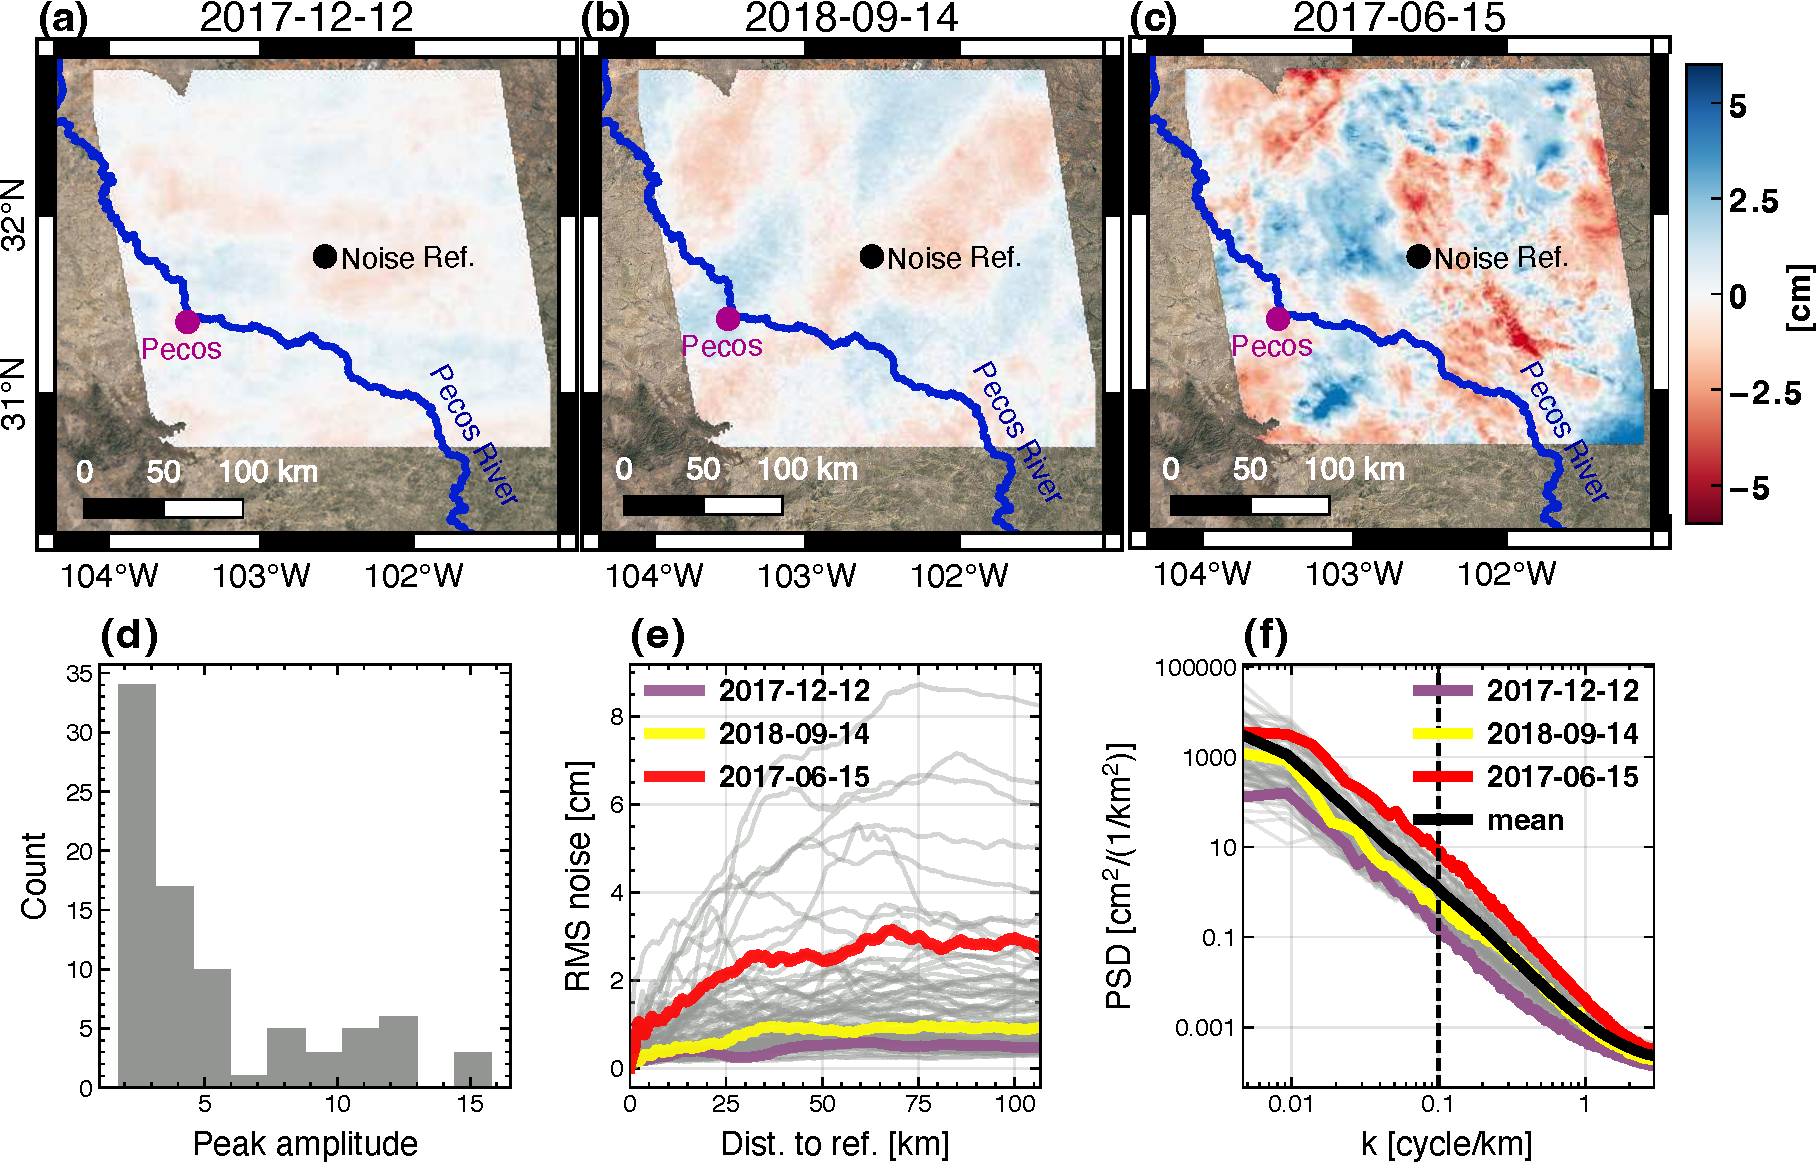
\includegraphics[width=0.98\linewidth]{figures/chapter6-blobs/figure5_noise_path78.png}
	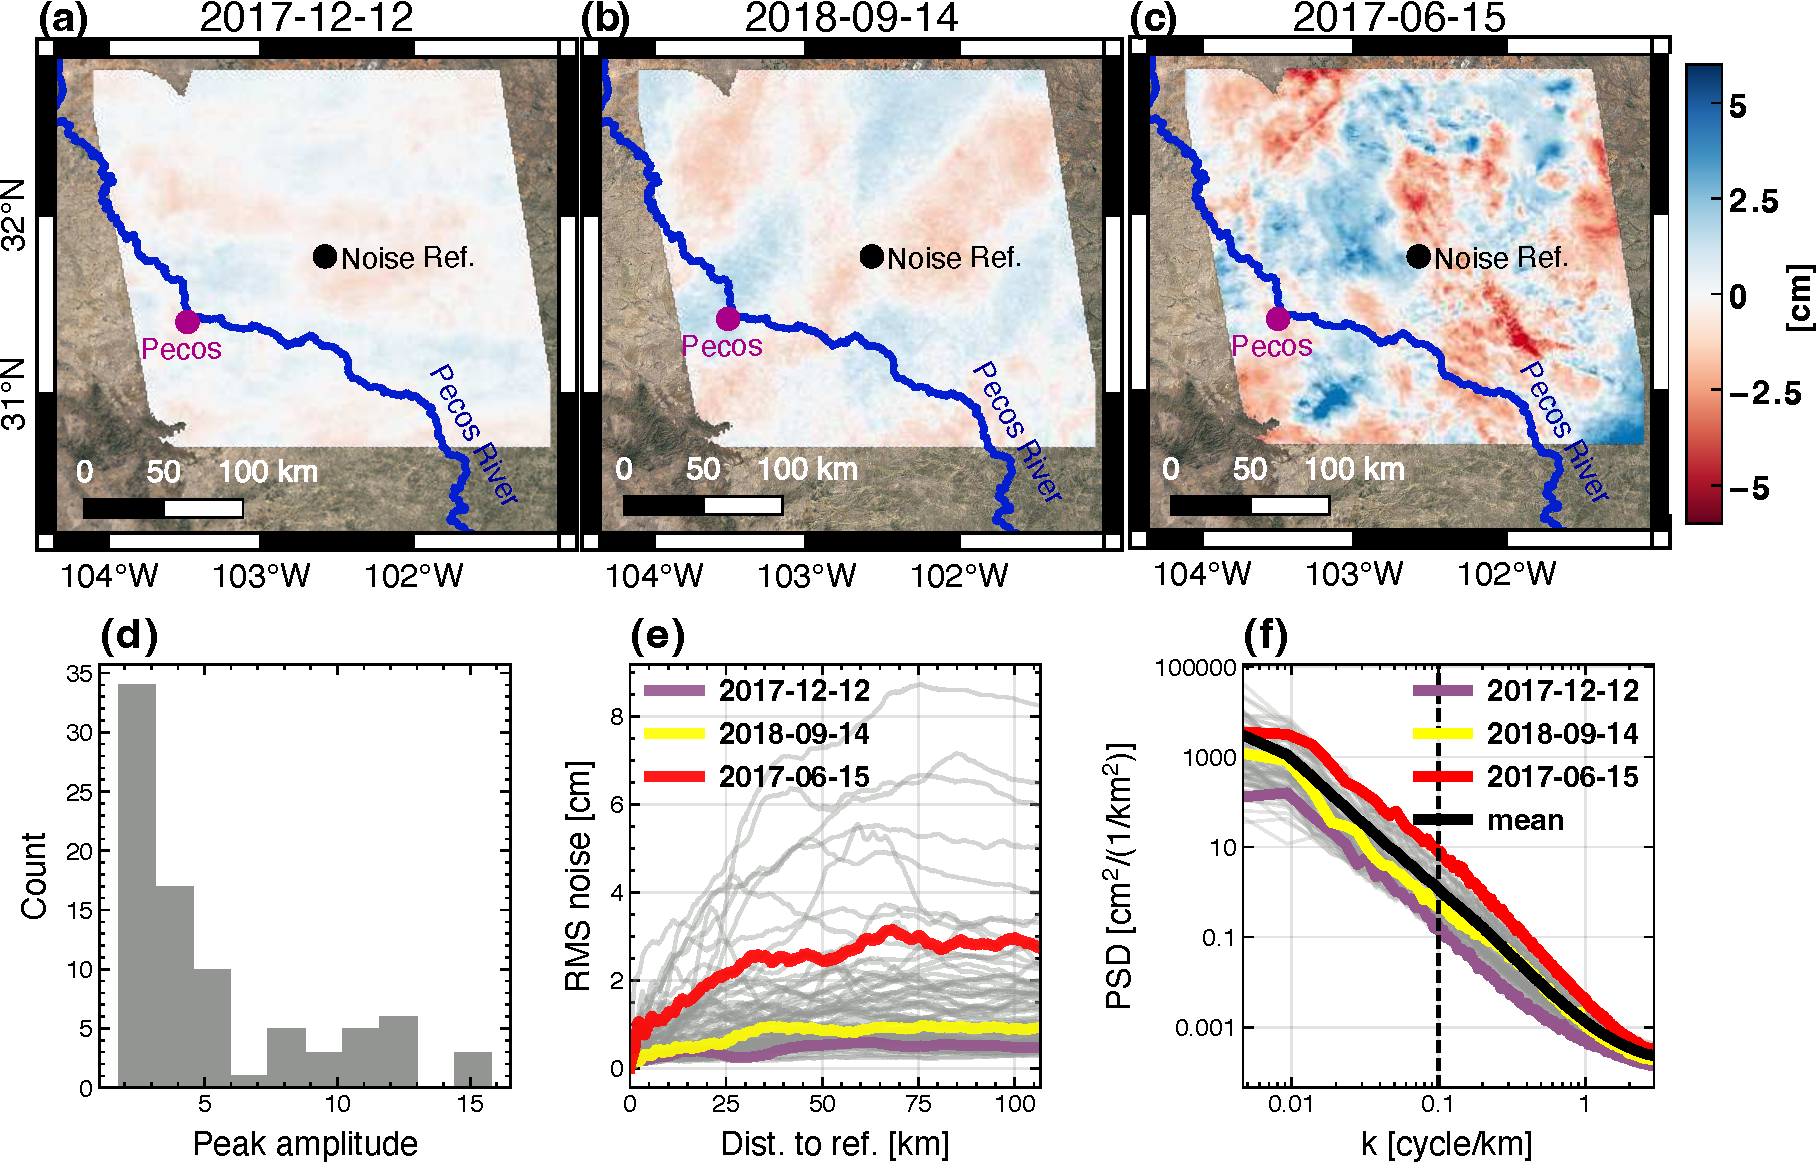
\includegraphics[width=0.98\linewidth]{figures/chapter6-blobs/figure5_noise_path78.pdf}
	\caption[Path 78 estimated tropospheric turbulence noise maps]{
		InSAR-estimated tropospheric turbulence noise maps for three Path 78 SAR acquisitions: (a) 2017-12-12 (up to 1.8 cm noise), (b) 2018-09-14 (up to 3.2 cm noise), and (c) 2017-06-15  (up to 12.6 cm noise).
		(d) The distribution of peak tropospheric noise magnitude (in centimeters), (e) the root mean squared value of tropospheric noise vs. distance from the center of the map, and (f) the estimated 1D PSDs for 84 Sentinel-1 Path 78 acquisitions used in this study. In panel (e) and (f), the color lines represent three SAR acquisitions (panel (a)-(c)) with different tropospheric noise levels. The black line in panel (f) represents the mean PSD of all 84 acquisitions.}
	\label{fig:results-noise}
\end{figure*}


The 1D PSDs for the 84 tropospheric turbulence noise maps give an alternative view of the distribution of noise power over different frequencies (Figure \ref{fig:results-noise} (f). For most spatial frequencies, the PSDs decay following the -8/3 power law described in previous studies \citep{Hanssen2001RadarInterferometryData, Onn2006ModelingWaterVapor}. This slope flattens at the low frequencies because we removed the quadratic phase in the noise solutions. The slope also flattens at high frequencies, where decorrelation noise introduces pixel-level variations in the noise map.
%\subsection{Simulated tropospheric turbulence noise and Uncertainty Quantification}



\begin{figure*}
	\centering 
	%\includegraphics[width=0.99\linewidth]{figures/chapter6-blobs/figure_results_simulation_kde.png}
	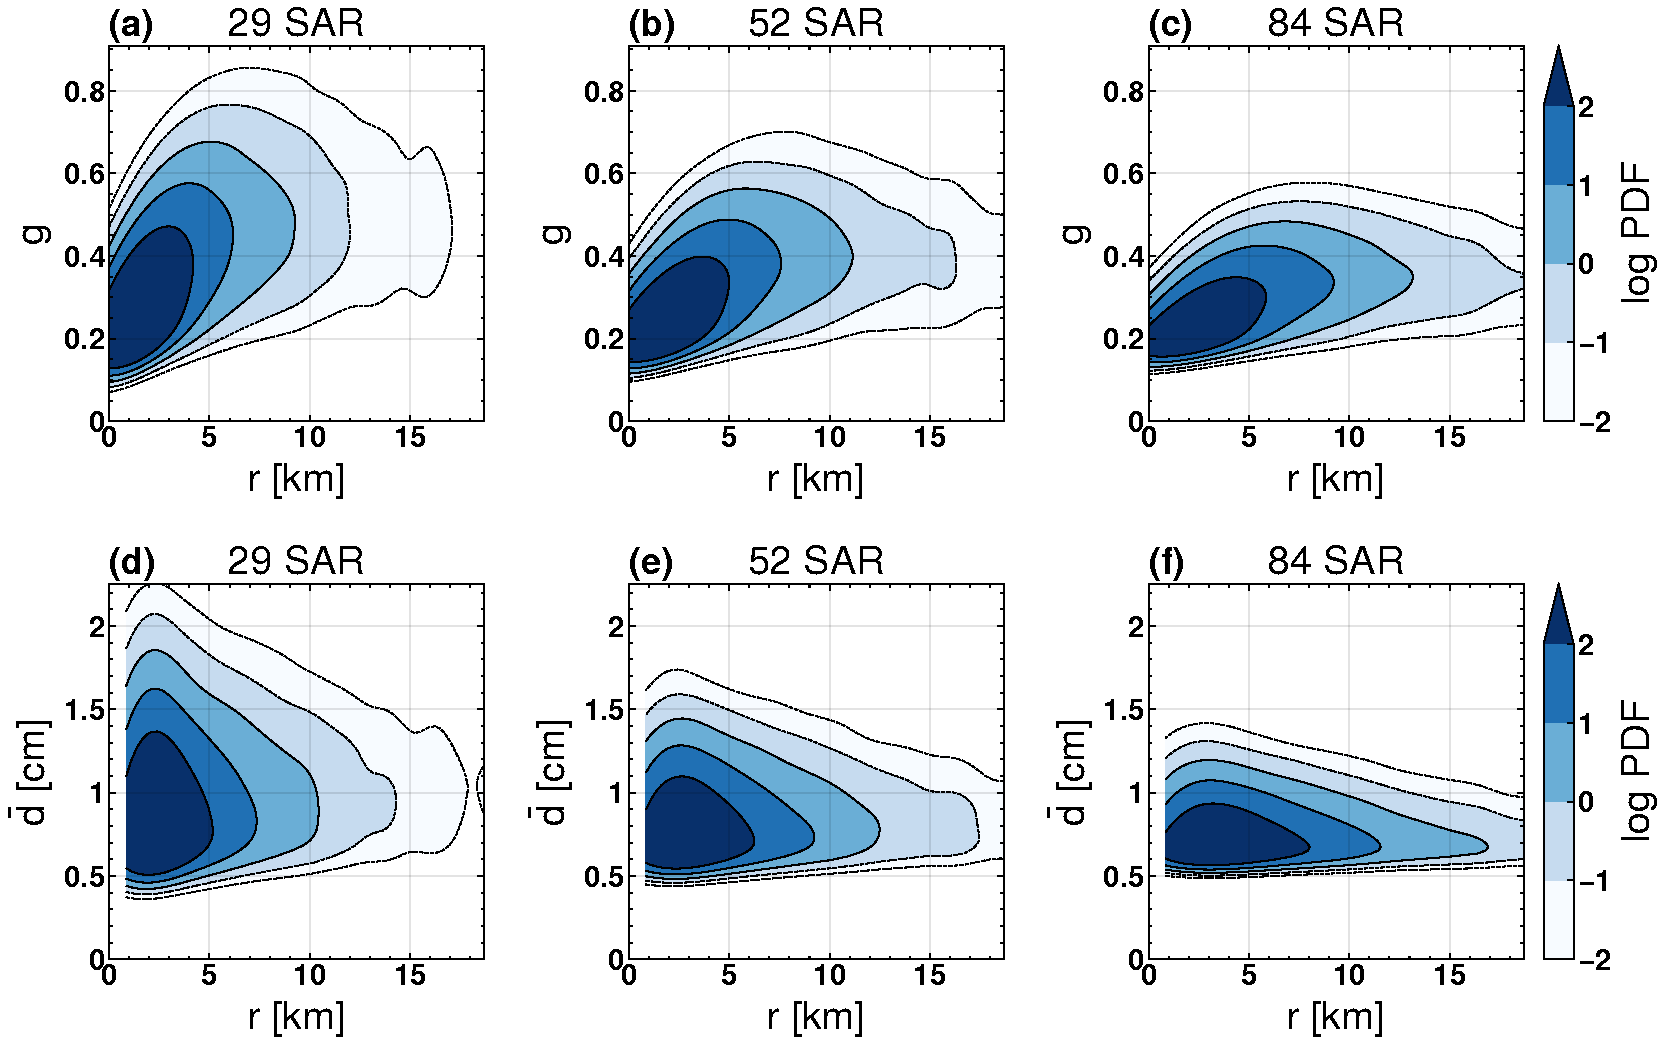
\includegraphics[width=0.99\linewidth]{figures/chapter6-blobs/figure_results_kde.pdf}
	\caption[Probability density function of detecting tropospheric noise blobs]{
		(a)-(c) Log Probability Density Function (PDF) of detecting tropospheric noise blobs as a function of feature size $r$ and filter response magnitude $|g|$ for three cumulative LOS deformation maps: November 2014 - January 2017 (29 SAR scenes from Path 78), November 2014 - January 2018 (52 SAR Scenes from Path 78), and November 2014 - January 2019 (84 SAR Scenes from Path 78).
		(d)-(f) Log Probability Density Function (PDF) of detecting tropospheric noise blobs as a function of feature size $r$ and deformation magnitude $|d|$ for the same three cumulative LOS deformation maps.
		The PDFs were generated from 2D histograms using a kernel density estimate (KDE) \citep{Scott2015MultivariateDensityEstimation}.
	}
	\label{fig:results-kde}
\end{figure*}

Using the mean 1D PSD shown in Figure \ref{fig:results-noise} (f), we simulated instances of tropospheric turbulence, and computed the empirical PDFs of the noise attributes for each deformation map (Figure \ref{fig:results-kde}).  Most of detected noise features have small radii ($r <$ 5 km). For the 29 SAR acquisition case, the noise features are unlikely to be larger 2 cm in magnitude or have a filter response stronger than 0.7 (Figure \ref{fig:results-kde} (a), (d)). For the 52 SAR acquisition case, the noise features are unlikely to be larger 1.5 cm in magnitude or have a filter response stronger than 0.6 (Figure \ref{fig:results-kde} (b), (e)). For the 84 SAR acquisition case, the noise features are unlikely to be larger 1.2 cm in magnitude or have a filter response stronger than 0.5 (Figure \ref{fig:results-kde} (c), (f)).
%(Figure \ref{fig:results-kde}(a-c)). The noise instances are spatially isotropic and contain many $\sim$3 cm blob-like features ranging from several km up to $\sim$100 km in length. As outlined in Section \ref{sec:site}, we computed three LOS deformation maps from 29,52, and 84 noise instances, and we recorded all detected noise features. The resulting histograms of ($g$ vs. $r$ and $\bar{d}$ vs. $r$) were smoothed using a kernel density estimate (KDE) \citep{Scott2015MultivariateDensityEstimation} to create 2D empirical probability density functions (PDFs) (Figure \ref{fig:results-kde}). As the number of SAR acquisitions increases to 52 (Figure \ref{fig:results-kde}(b),(e)) and 84 (Figure \ref{fig:results-kde}(c),(f)), the amplitudes of detected noise features decreases for all $r$.
Note that the maximum and minimum sizes of detected features in Figure \ref{fig:results-kde} (d)-(f) are determined by the choice of maximum and minimum kernel sizes $\sigma_{max}$ and $\sigma_{max}$ in our automatic detection algorithm. By imposing the prior knowledge that oil and gas-production related deformation bowls are unlikely to be larger than 30-40 km in the Permian Basin \citep{Staniewicz2020InsarRevealsComplex}, $\sigma_{max}$ was set so that the maximum detected feature radius $r$ was approximately 20 km. Thus, large-scale tropospheric noise features ($>$ 20 km) were not recorded in the noise simulations.
%\subsection{West Texas Detected Deformation}



\begin{figure*}	[h]
	\centering 
	%\includegraphics[width=0.98\linewidth]{figures/chapter6-blobs/figure_results_detections_vert.png}
	%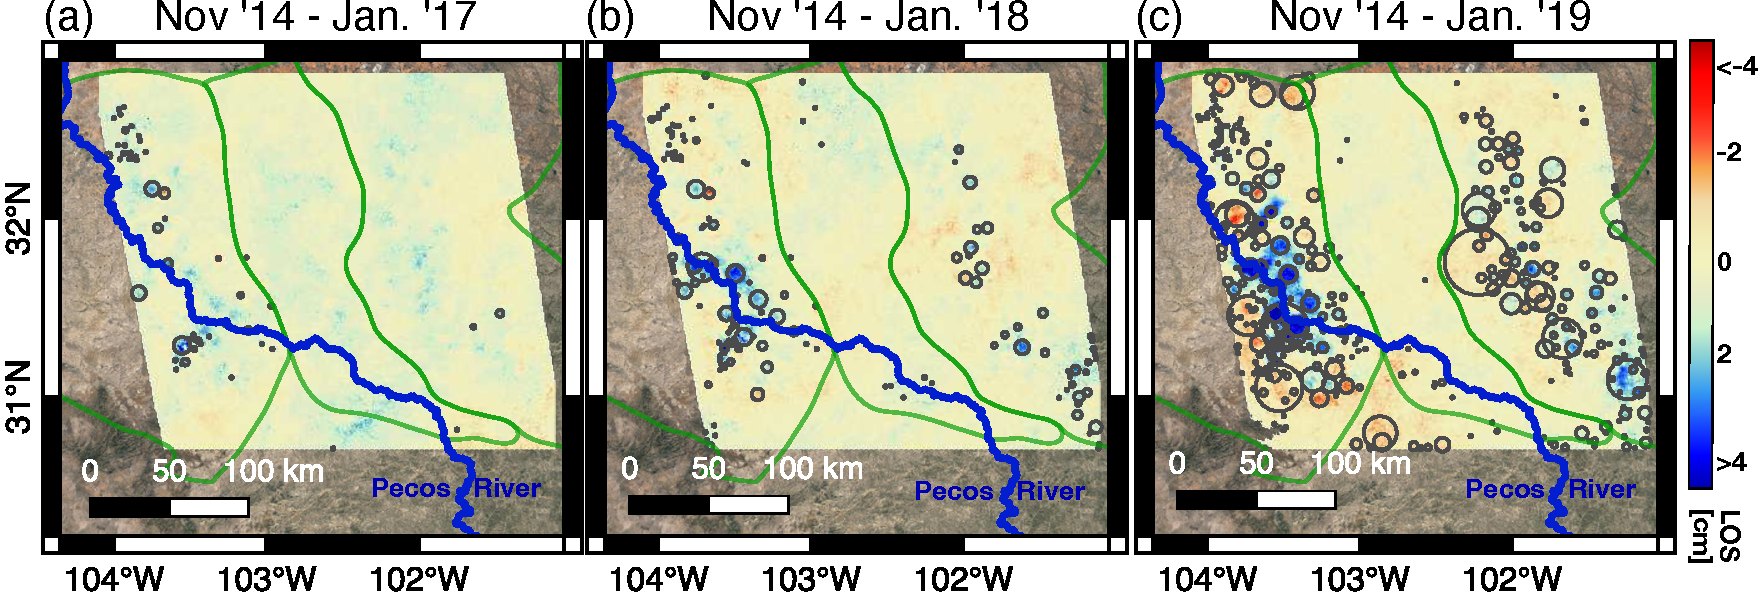
\includegraphics[width=0.98\linewidth]{figures/chapter6-blobs/figure_results_blobs_path78.png}
	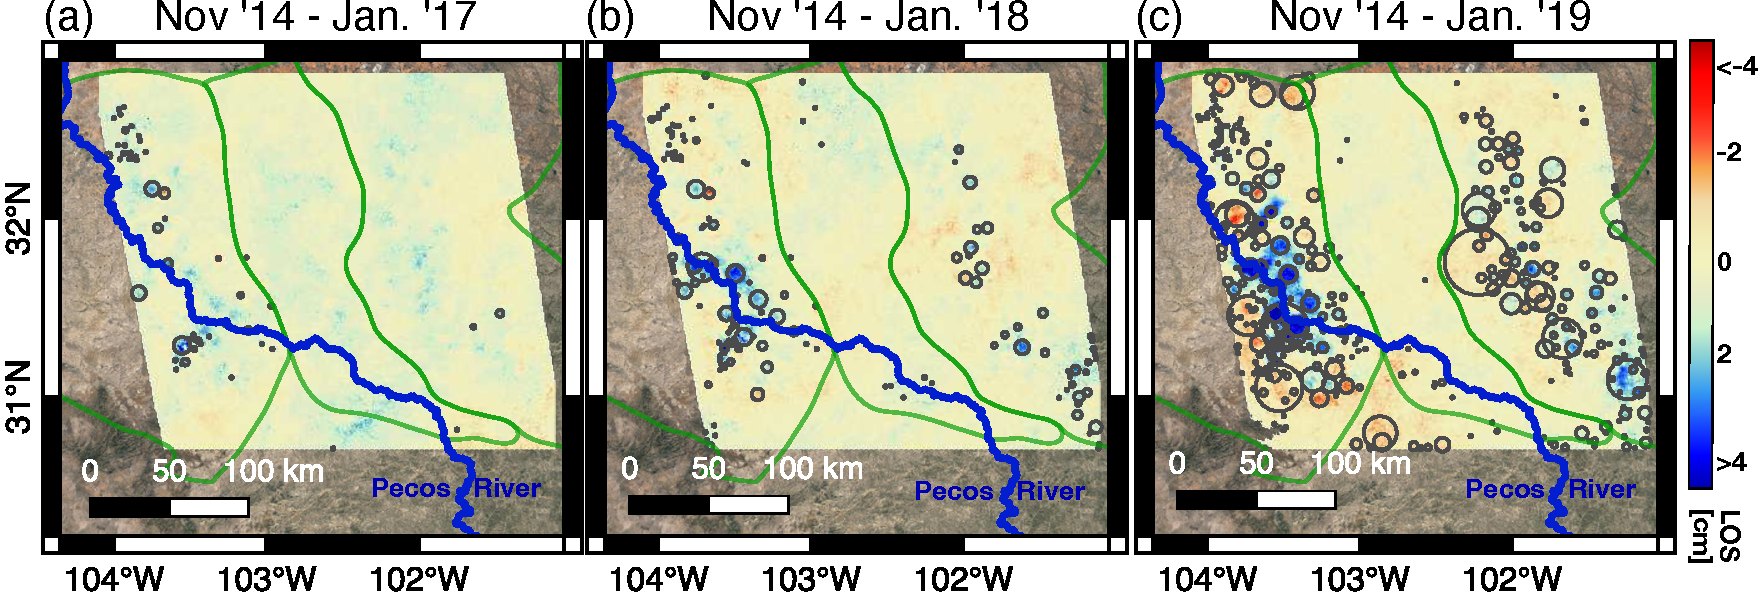
\includegraphics[width=0.98\linewidth]{figures/chapter6-blobs/figure_results_blobs_path78.pdf}
	\caption[Detected deformation features for Path 78]{
		Detected deformation features (gray circles) from the three Path 78 cumulative LOS deformation maps. Features with more than 5\% chance of being noise for their radius, according to either the filter magnitude or image magnitude PDFs (Figure \ref{fig:results-kde}), have been removed. Green lines correspond the boundaries of the Delaware Basin, Central Basin Platform, and Midland Basin from west to east.
		% Not shown are features which, given their radius, have with more than 5\% chance of being noise according to either the filter magnitude or image magnitude PDFs (Figure \ref{fig:results-kde}). 
	}
	\label{fig:results-detections}
\end{figure*}


Using the empirical PDFs of the noise attributes, we removed detections with more than 5\% chance of being noise from three Path 78 cumulative deformation maps (Figure \ref{fig:results-detections}). We identified 57 deformation features in the Nov. 2014-Jan. 2017 cumulative deformation map, 147 features in the Nov. 2014-Jan. 2018 map, and 268 features in the Nov. 2014-Jan. 2019 map. The increasing number of detected deformation features is due to (1) the oil and gas production rate experienced a sharp rise over the study period \citep{Staniewicz2020InsarRevealsComplex}; and (2) a larger number of SAR acquisitions reduces the noise level in the InSAR cumulative deformation solutions.



The detected features are mainly clustered in regions within the Midland Basin and the Delaware Basin. Here oil production and wasterwater injection caused many centimeter-level subsidence and uplift features. In the Southern Delaware Basin, the observed linear deformation features parallel the inferred favorable fault plane orientation proposed by \citep{LundSnee2018StateStressPermian}, and they align with a cluster of recent shallow earthquakes cataloged by TexNet \citep{Savvaidis2019TexnetStatewideSeismological}. Very few deformation features were detected in the Central Basin Platform, where oil and gas are mostly produced from conventional reservoirs and the subsurface pressure was well maintained.


\begin{figure*}[h]
	\centering 
	% vertical version:
	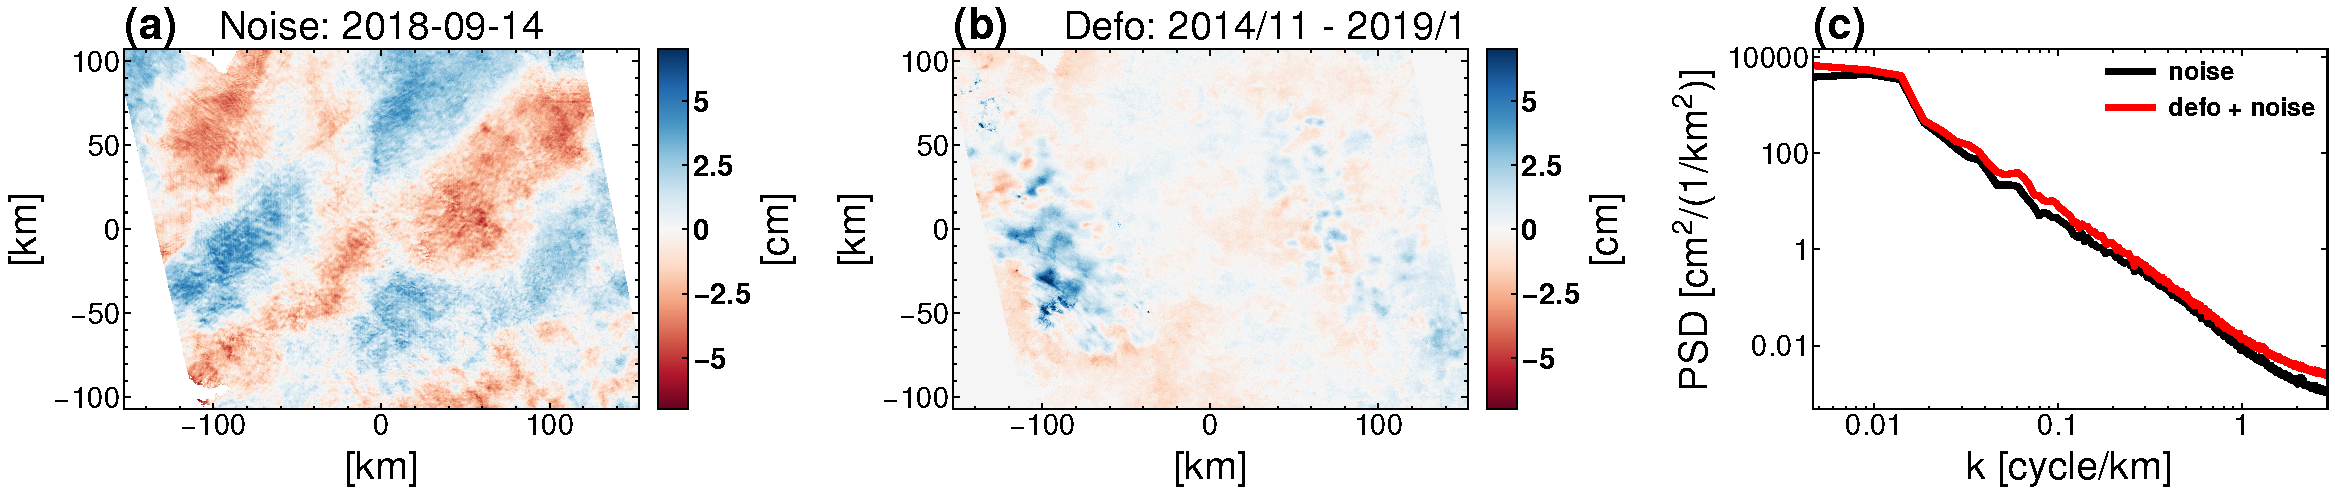
\includegraphics[width=0.98\linewidth]{figures/chapter6-blobs/figure_discussion_residual_defo.pdf}
	%\includegraphics[width=0.98\linewidth]{figures/chapter6-blobs/figure_discussion_residual_defo_horizontal.pdf}
	\caption[Effect of residual deformation on tropospheric noise PSD]{
		(a) InSAR-estimated tropospheric noise map for the Path 78 SAR acquisition 2018-09-14. 
		(b) Cumulative LOS deformation from Nov. 2014 to Jan. 2019 as inferred from Sentinel-1 Path 78 InSAR data.
		(c) 1D PSDs derived from the tropospheric noise map (black) and the tropospheric noise plus deformation map (red).
	}
	\label{fig:discussion-residual-defo}
\end{figure*}


For the West Texas case, the residual deformation term $  \frac{1}{N-1}  \sum  \Delta d_{n,k} $ in Equation \eqref{eq:avg-ifg} does not significantly influence our noise simulations. To demonstrate this, Figure \ref{fig:discussion-residual-defo} (a) shows the tropospheric noise estimates on a quiet atmospheric date (2018-09-04) and Figure  \ref{fig:discussion-residual-defo} (b) shows the cumulative LOS deformation solution between  Nov. 2014 and Jan. 2019. The 1D PSDs for the noise-only map and the noise plus deformation map are very similar (Figure \ref{fig:discussion-residual-defo} (c)). This is because the total integrated power of the noise map is five times larger than the total power of the deformation map. Since the residual deformation contribution in Equation \eqref{eq:avg-ifg}, $ \frac{1}{N-1}  \sum  \Delta d_{n,k} $, is much less than the total cumulative deformation over the entire study period, we conclude that this term in the tropospheric noise estimates has negligible effects on the detection confidences derived from the noise simulations.



\subsection{Path 85 Detections}
\label{subsec:discussion-path85}



\begin{figure*}[h]
	\centering 
	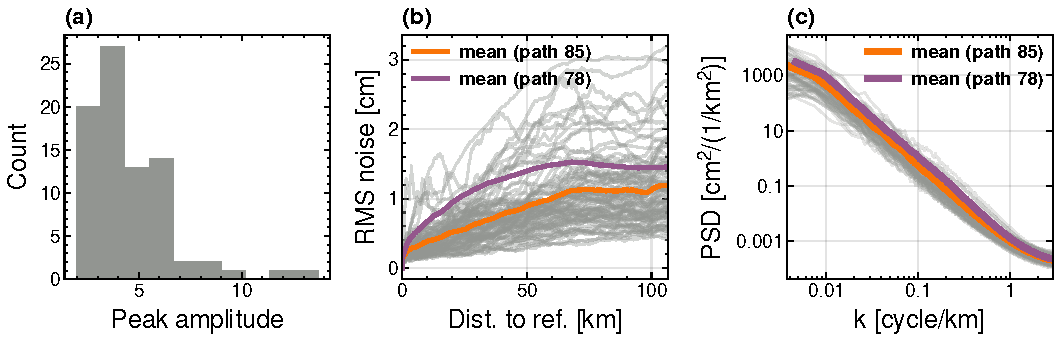
\includegraphics[width=0.98\linewidth]{figures/chapter6-blobs/figure_discussion_path85_plots.pdf}
	\caption[Path 85 estimated tropospheric turbulence noise maps]{
		(a) The distribution of peak tropospheric noise magnitude (in centimeters), (b) the root mean squared value of tropospheric noise vs. distance from the center of the map, and (c) the estimated 1D PSDs for 81 Sentinel-1 Path 85 acquisitions used in this study. In panel (b) and (c), the color lines represent the average estimates for Path 85 (orange) and Path 78 (purple).
	}
	\label{fig:discussion-noise-85}
\end{figure*}


\begin{table}[h]
	\centering
	\caption{Tropospheric noise characteristics for Sentinel-1 Path 85 and Path 78 data over West Texas}
	\begin{tabular}{lrr}
		\toprule
		{} &  Path 78 &  Path 85 \\
		\midrule
		Average Variance [cm$^2$]             &     1.38 &     0.78 \\
		Variance of the Noisiest Date [cm$^2$] &    10.68 &     3.74 \\
		Average Peak Amplitude [cm]            &     5.36 &     4.58 \\
		Peak Amplitude of the Noisiest Date [cm]         &    15.81 &    13.72 \\
		%\midrule
		%Detected features with confidence $p<0.05$ & & \\
		%\midrule
		%Through Jan '17 & 48 & 58 \\
		%Through Jan '18 & 102 & 130 \\
		%Through Jan '19 & 256 & 343 \\
		\bottomrule
	\end{tabular}
	\label{tab:path85-compare}
\end{table}

Similar to the ascending Path 78 results, approximately 50\% of descending Path 85 scenes were acquired in quiet atmospheric conditions with a maximum noise level under 4 cm (Figure \ref{fig:discussion-noise-85} (a)). However, only 2 out of 81 descending scenes were acquired in strong turbulent noise conditions (a maximum noise level over 10 cm), while 14 out of the 84 ascending scenes were acquired in such conditions. We also found that the average tropospheric noise level is lower for Path 85 than Path 78 (Figure \ref{fig:discussion-noise-85} (b)-(c)). For example, the mean absolute tropospheric noise is 50\% larger for Path 78 than Path 85 at 50 km, and the mean noise PSD is more than 2 times larger for Path 78 than Path 85 at a spatial frequency of 0.1 cycles/km. We summarized the noise statistics of Path 78 and Path 85 acquisitions in Table \ref{tab:path85-compare}. The differences are due to the fact that Sentinel-1 satellites acquire Path 78 data over West Texas at 7:50 p.m. local time, and Path 85 data at 6:55 a.m local time. The expected tropospheric noise signatures are typically more substantial in late afternoon than early morning. 




Our algorithm identified similar numbers of blob features from the ascending and descending cumulative LOS deformation maps that span the same period of interest. Because the tropospheric noise level is generally lower in Path 85 data, fewer Path 85 detections need to be removed for having $>5\%$ chance of being tropospheric noise. As a result, we detected more deformation features from the Path 85 dataset than the Path 78 dataset. It is also worth noting that the number of detected deformations in both paths increases substantially over the study period. This is consistent with the overall rise in oil production within the Permian Basin during this time period (Figure \ref{fig:discussion-oil-blob-count}) .




\begin{figure*}
	\centering 
	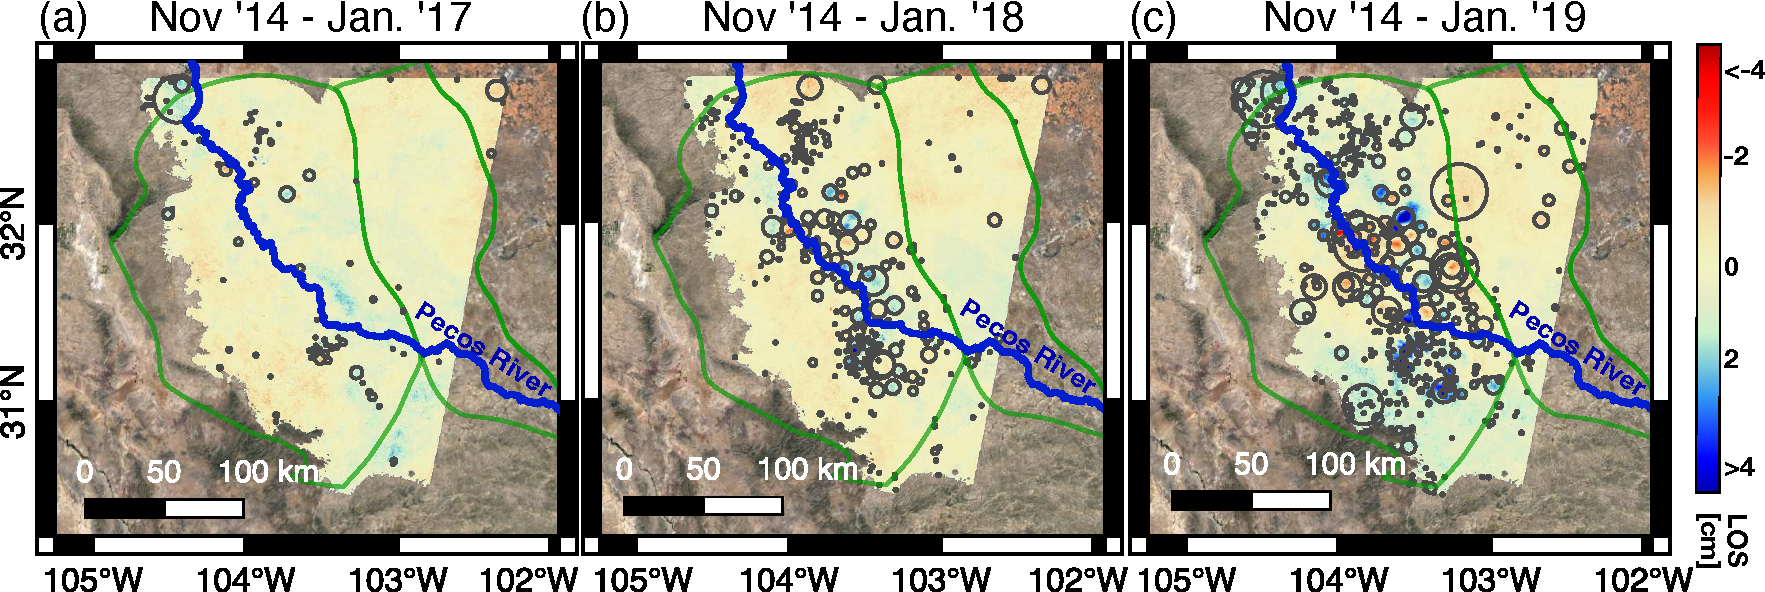
\includegraphics[width=0.98\linewidth]{figures/chapter6-blobs/figure_discussion_blobs_combined_path85.pdf}
	\caption[Detected deformation features for Path 85]{
		Detected deformation features (gray circles) from the three Path 85 cumulative LOS deformation maps. Features with more than 5\% chance of being noise for their radius, according to either the filter magnitude or image magnitude PDFs (Figure \ref{fig:results-kde}), have been removed. Green lines illustrate the boundaries of the Delaware Basin and Central Basin Platform, from west to east.
		%The blobs with more than 5\% chance to be noise, given their radius within the filter magnitude and image magnitude PDFs
	}
	\label{fig:discussion-detections-85}
\end{figure*}


\begin{figure}
	\centering 
	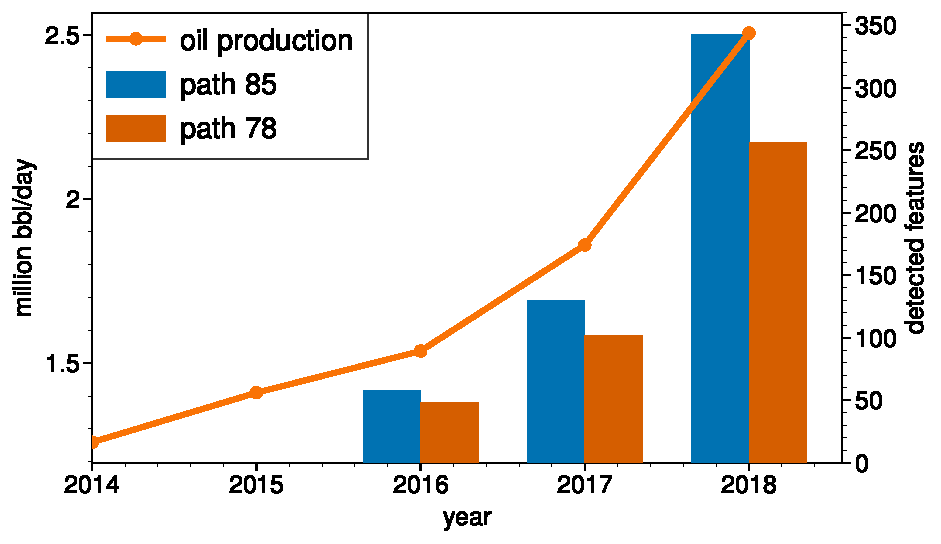
\includegraphics[width=.85\linewidth]{figures/chapter6-blobs/figure_discussion_oil_vs_blob_count_1col.pdf}
	\caption[Detected deformation features vs daily Permian Basin oil production]{
		The number of deformation features ($<$ 5\% chance of being tropospheric noise) detected from three Path 78 cumulative LOS deformation maps (Figure \ref{fig:results-detections}) and three Path 85 cumulative LOS deformation maps (Figure \ref{fig:discussion-detections-85}). Only detections from the overlapping region of the two paths are counted. The Permian Basin average daily oil production from 2014 and 2018 is shown as the orange line.
	}
	\label{fig:discussion-oil-blob-count}
\end{figure}
